%% Background
\chapter{Background}
\label{chap:background}

\section{Font Selection}

This section explores some important background information about the history and current state of font selection tools. Comparing one of the earliest font selection interfaces---from the built-in word processor on the 1981 Xerox Star---to the typical font selection interfaces on Google Docs, Microsoft Word, and Apple Pages, it is evident that little progress has been made in the way we select fonts. Nevertheless, there has been some recent innovation in typeface selection interfaces, and we explore some of these new approaches---specifically the new language-based font selection models of the Google Fonts website and Canva, a popular online graphic design tool. We additionally discuss the difficulty of creating language-based font selection tools. Lastly, we provide an analogue between font selection interfaces and the much more diverse field of color selection, another common selection in graphic design, to envision alternative modeling schema for font selection.

\subsection{Lack of Development in Font Selection Interfaces}

Surprisingly little progress has been made in the past several decades on user font selection. Figure \ref{fig:xerox-star} shows the font selection interface on the 1981 Xerox Star, one of the earliest personal computers to include a multi-font word processor. This interface will probably look familiar to a modern user: it provides control over font size; bold, italic, underline, and strikethrough toggles; superscript and subscript options; and, importantly, a scrollable list of fonts to choose between. Compared to the modern font selection interfaces shown in Figure \ref{fig:font-selectors}, the only significant difference over this 44-year gap is the alphabetization of the font selector list; otherwise, these interfaces are practically identical. While there are many beneficial aspects of this interface---control over size, boldness, and other useful dimensions of typeface---the list-based typeface selector has become increasingly unfit for the task of font selection. Whereas the Xerox Star provided its users with a small number of typefaces to choose between, today the number of individual typefaces available to users (although impossible to enumerate exactly) almost certainly exceeds 300,000 \cite{cheng2006}. It is not feasible for a user to scroll through this many typefaces when making a font selection. Additionally, this interface provides little guidance about style: in an alphabetized list, there is no particular relationship between nearby fonts, or any capability for style-based search. This leads users to find a few fonts they like and stick with them, rather than explore the wide variety available to them. Without a better tool for navigating the many dimensions of typeface style, this will remain the case.

% from Designing the Xerox “Star” User Interface, Byte, issue 4, 1982
\begin{figure}
    \centering
    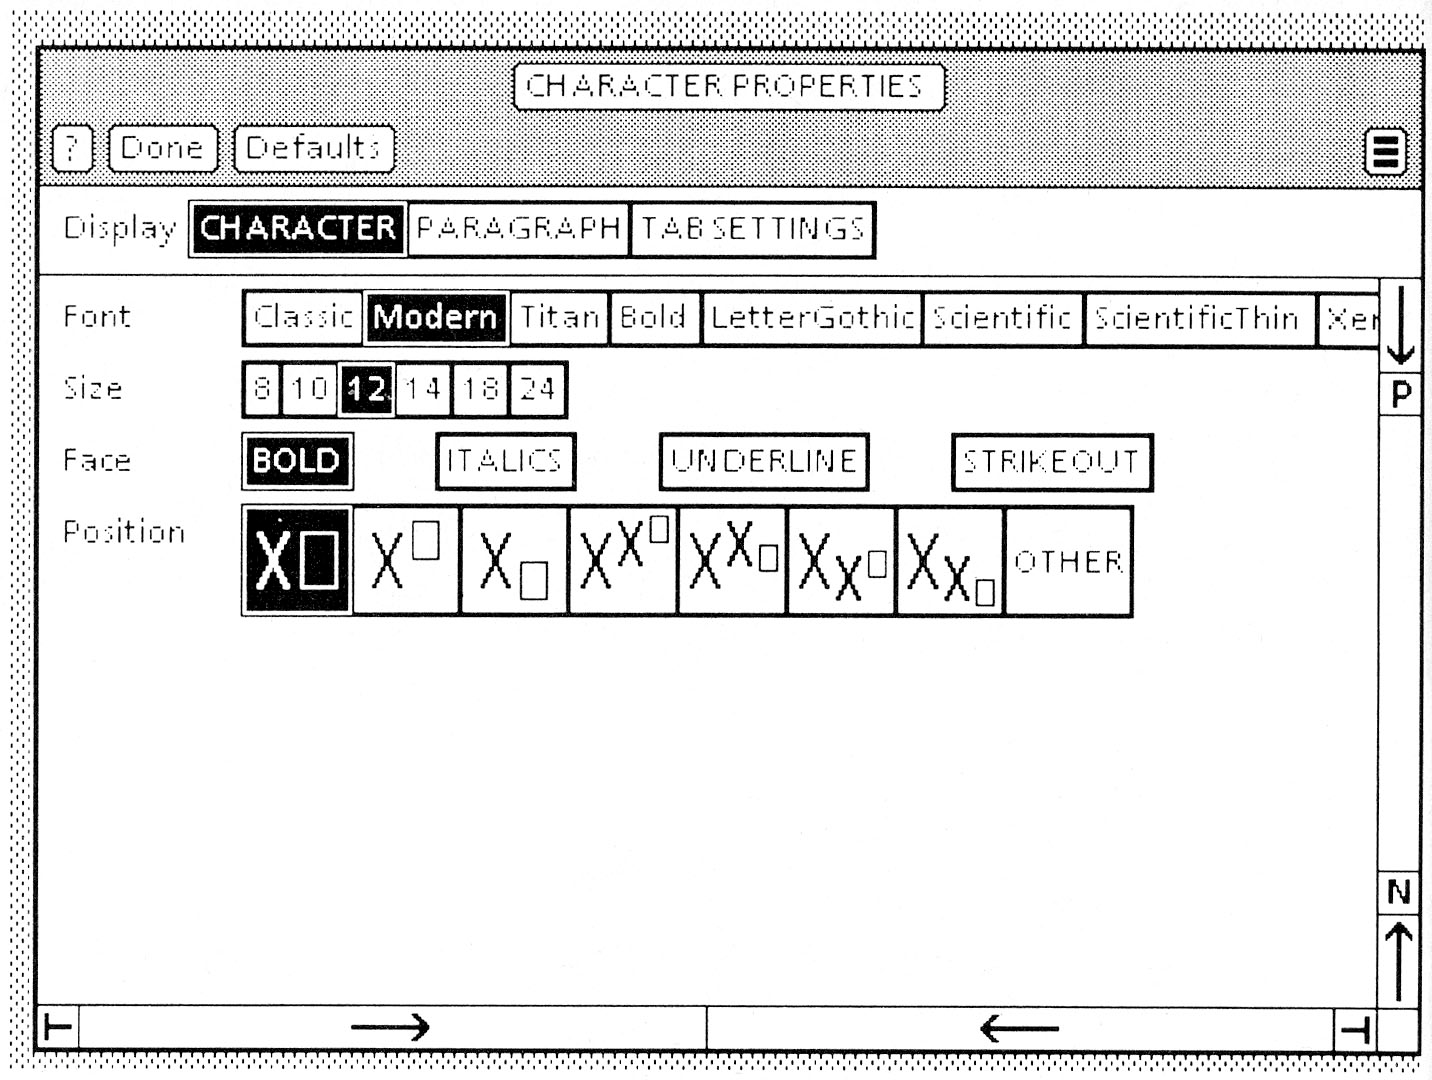
\includegraphics[width=.8\textwidth]{images/xerox-star.png}
    \caption{Font selection interface in Xerox Star (1981)}
    \label{fig:xerox-star}
\end{figure}

O'Donovan et al.\ \cite{odonovan2014} lists several reasons for the difficulty of developing font selection tools. The first issue, as discussed above, is the sheer number of available fonts. ``Most computers are now equipped with hundreds of fonts,'' they note, while online resources provide access to hundreds of thousands. Another issue is a lack of obvious ways to categorize fonts in a manner which corresponds to user goals. While there exist broad categories like Serif, Sans Serif, and Handwritten, these must be manually designated on a per-font basis, and they are not necessarily helpful to every user. A college student, for example, might know to choose a Serif font for their paper to convey an academic mood—or, more practically, to fulfill certain departmental design expectations—however another user, looking to design a new logo for their coffee shop, might not find the distinction between Serif, Sans Serif, and Handwritten typeface particularly useful or informative. Typical users lack the tools, given the current state of font selector interfaces, to properly consider the wide range of typefaces and confidently choose the right font—one of the most fundamental decisions in effective text-based graphic design. Finally, users vary in their font selection goals. One user may be looking to identify the font they saw on a store sign or a brochure—or to find a free-to-use font which is similar to a commercial one they have identified---while another may be looking to match a particular mood, or to choose a font that fits well with the rest of their document. A third may simply be exploring a large set of fonts like Adobe TypeKit or Google Fonts, curious to find new, exciting typefaces. O'Donovan et al.\ argue—and we agree—that current methods of font selection fall short on these issues. Given the growing number of fonts available to the modern user, a better, more useful system for typeface selection is long overdue.

% own screenshots
\begin{figure}
    \centering
    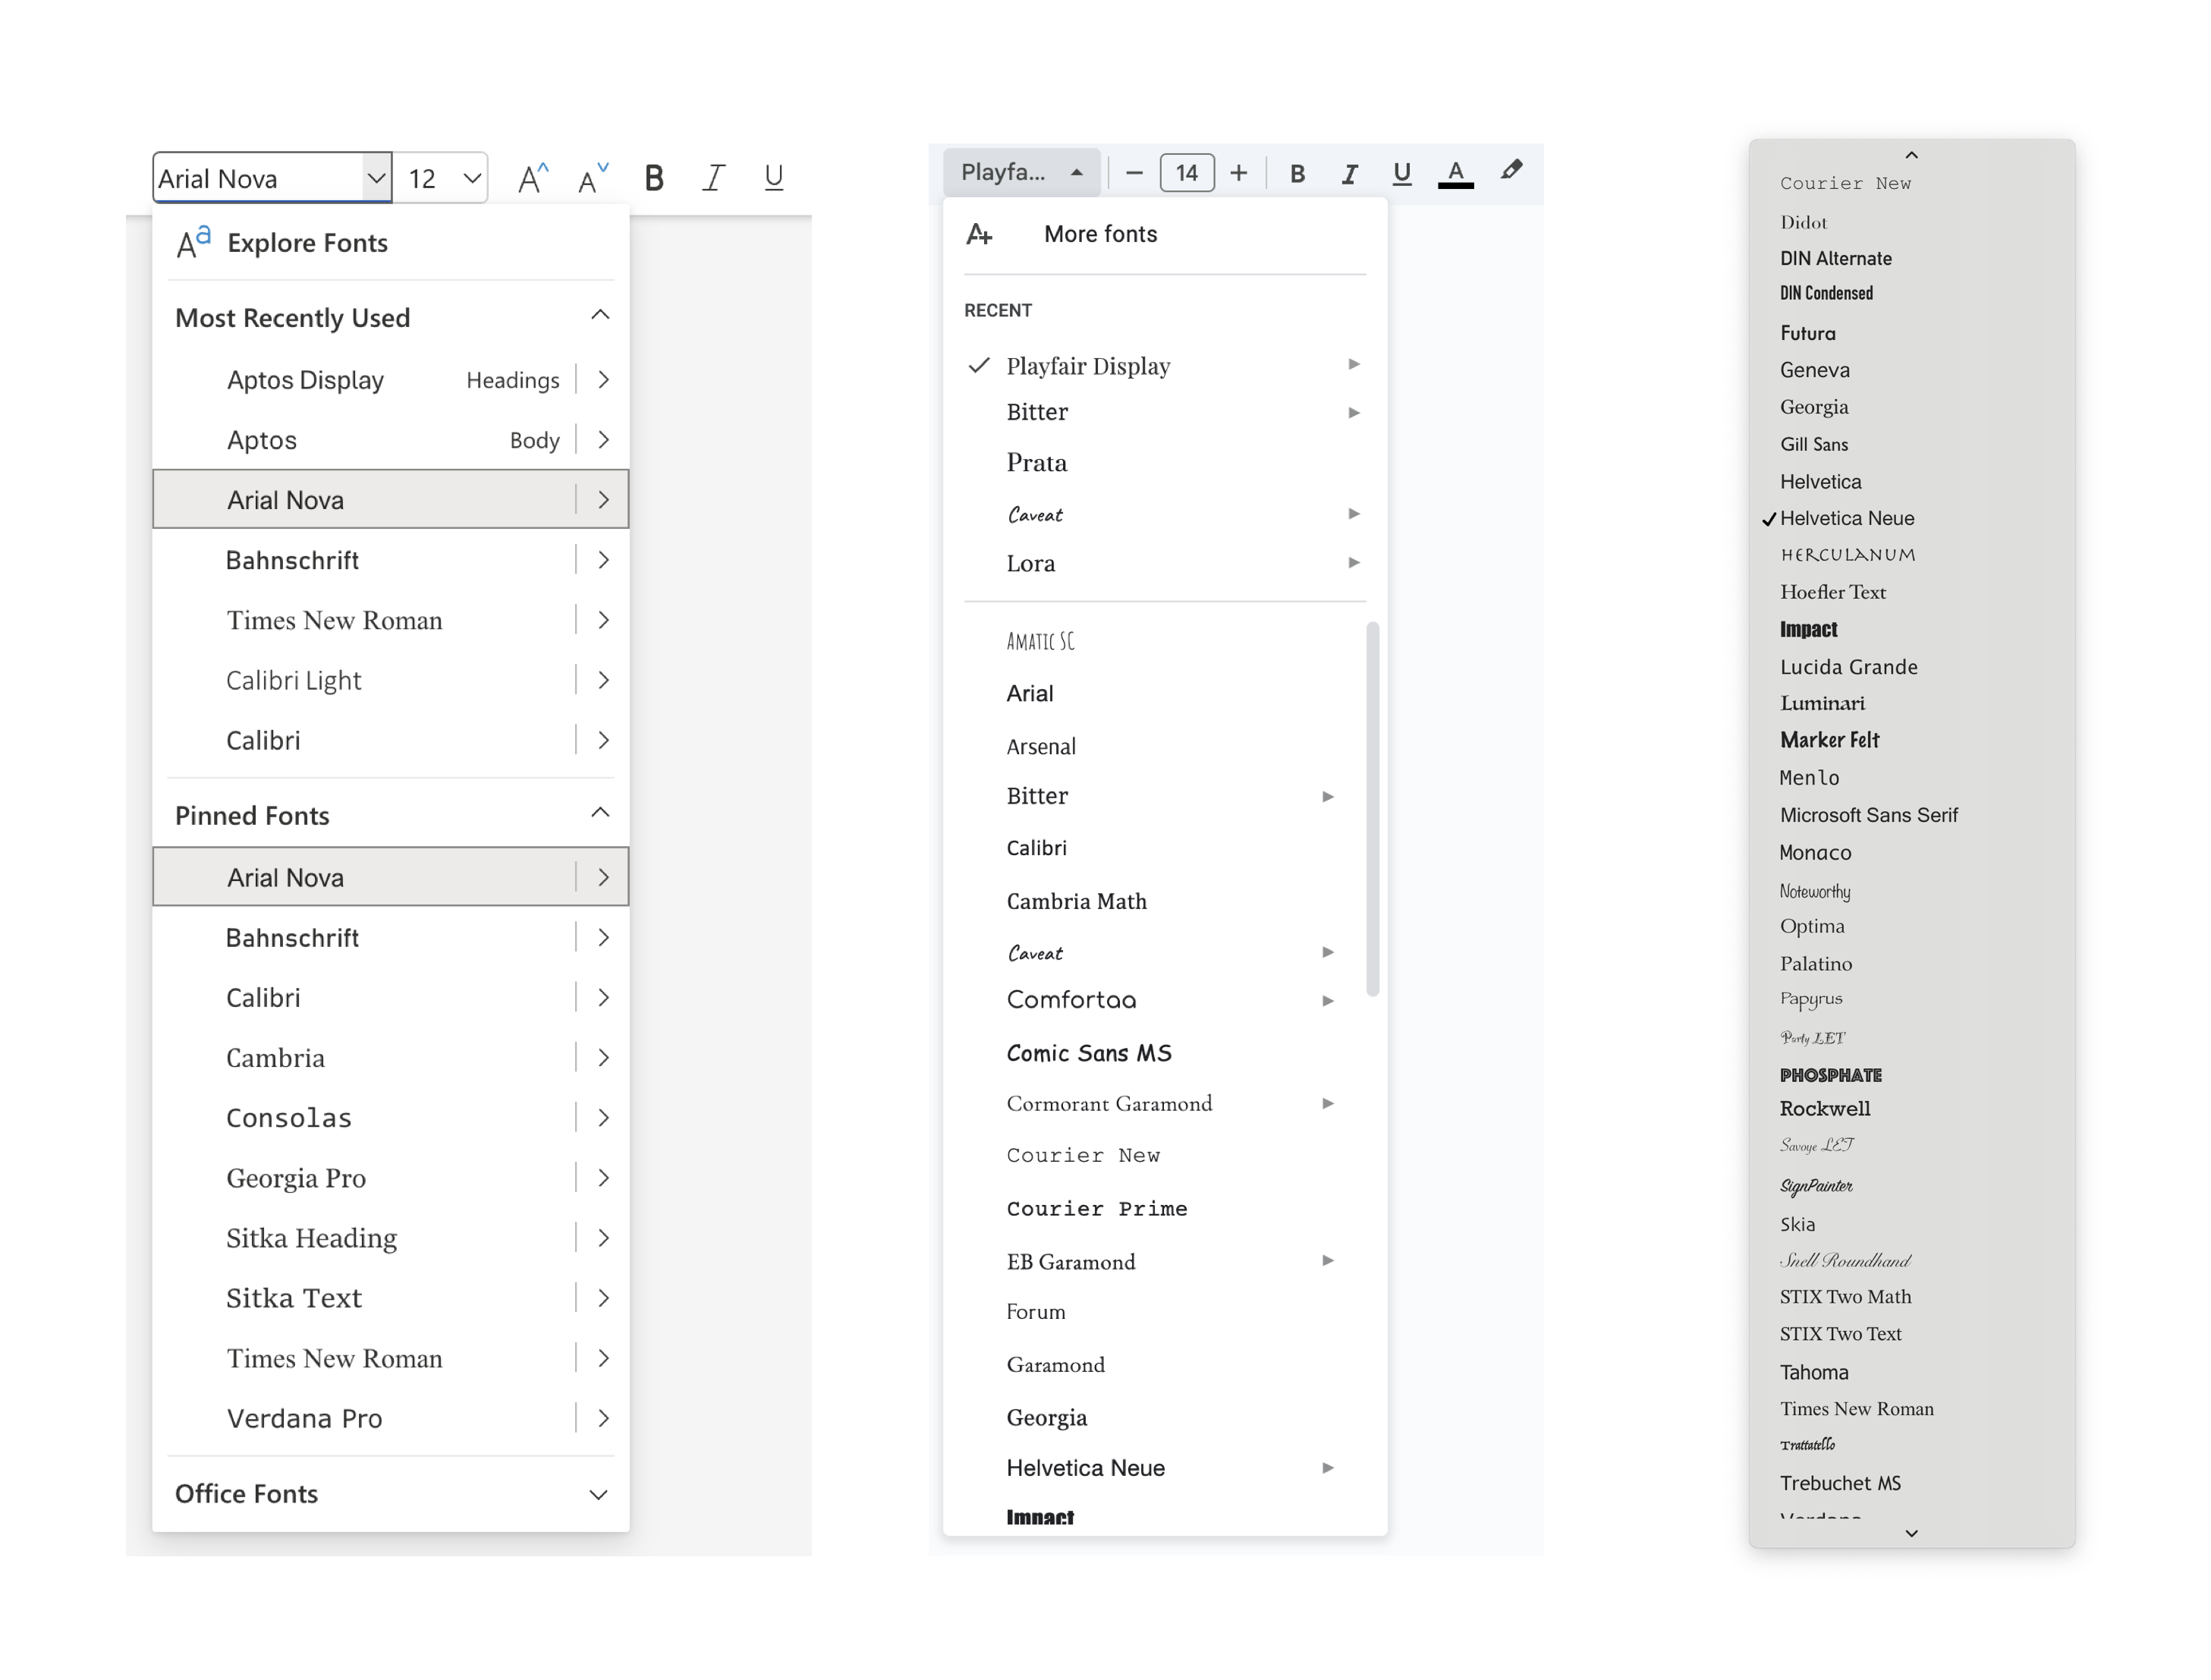
\includegraphics[width=1\textwidth]{images/font-selectors.png}
    \caption{Current font selection interfaces in Microsoft Word, Google Docs, and Apple Pages}
    \label{fig:font-selectors}
\end{figure}

\subsection{Font Selection Innovation} \label{font-selection-innovation}

There has been some limited progress, in recent years, in the field of font selection interfaces. Specifically, both Google Fonts and Canva, a popular online graphic design tool, have experimented with language-based font selection tools. Both of these interfaces break from the common list-based font selection tool, but both also have some significant drawbacks and flaws. This section will explore these two novel font selection interfaces and their respective contributions.

% own screenshots
\begin{figure}[H]
    \centering
    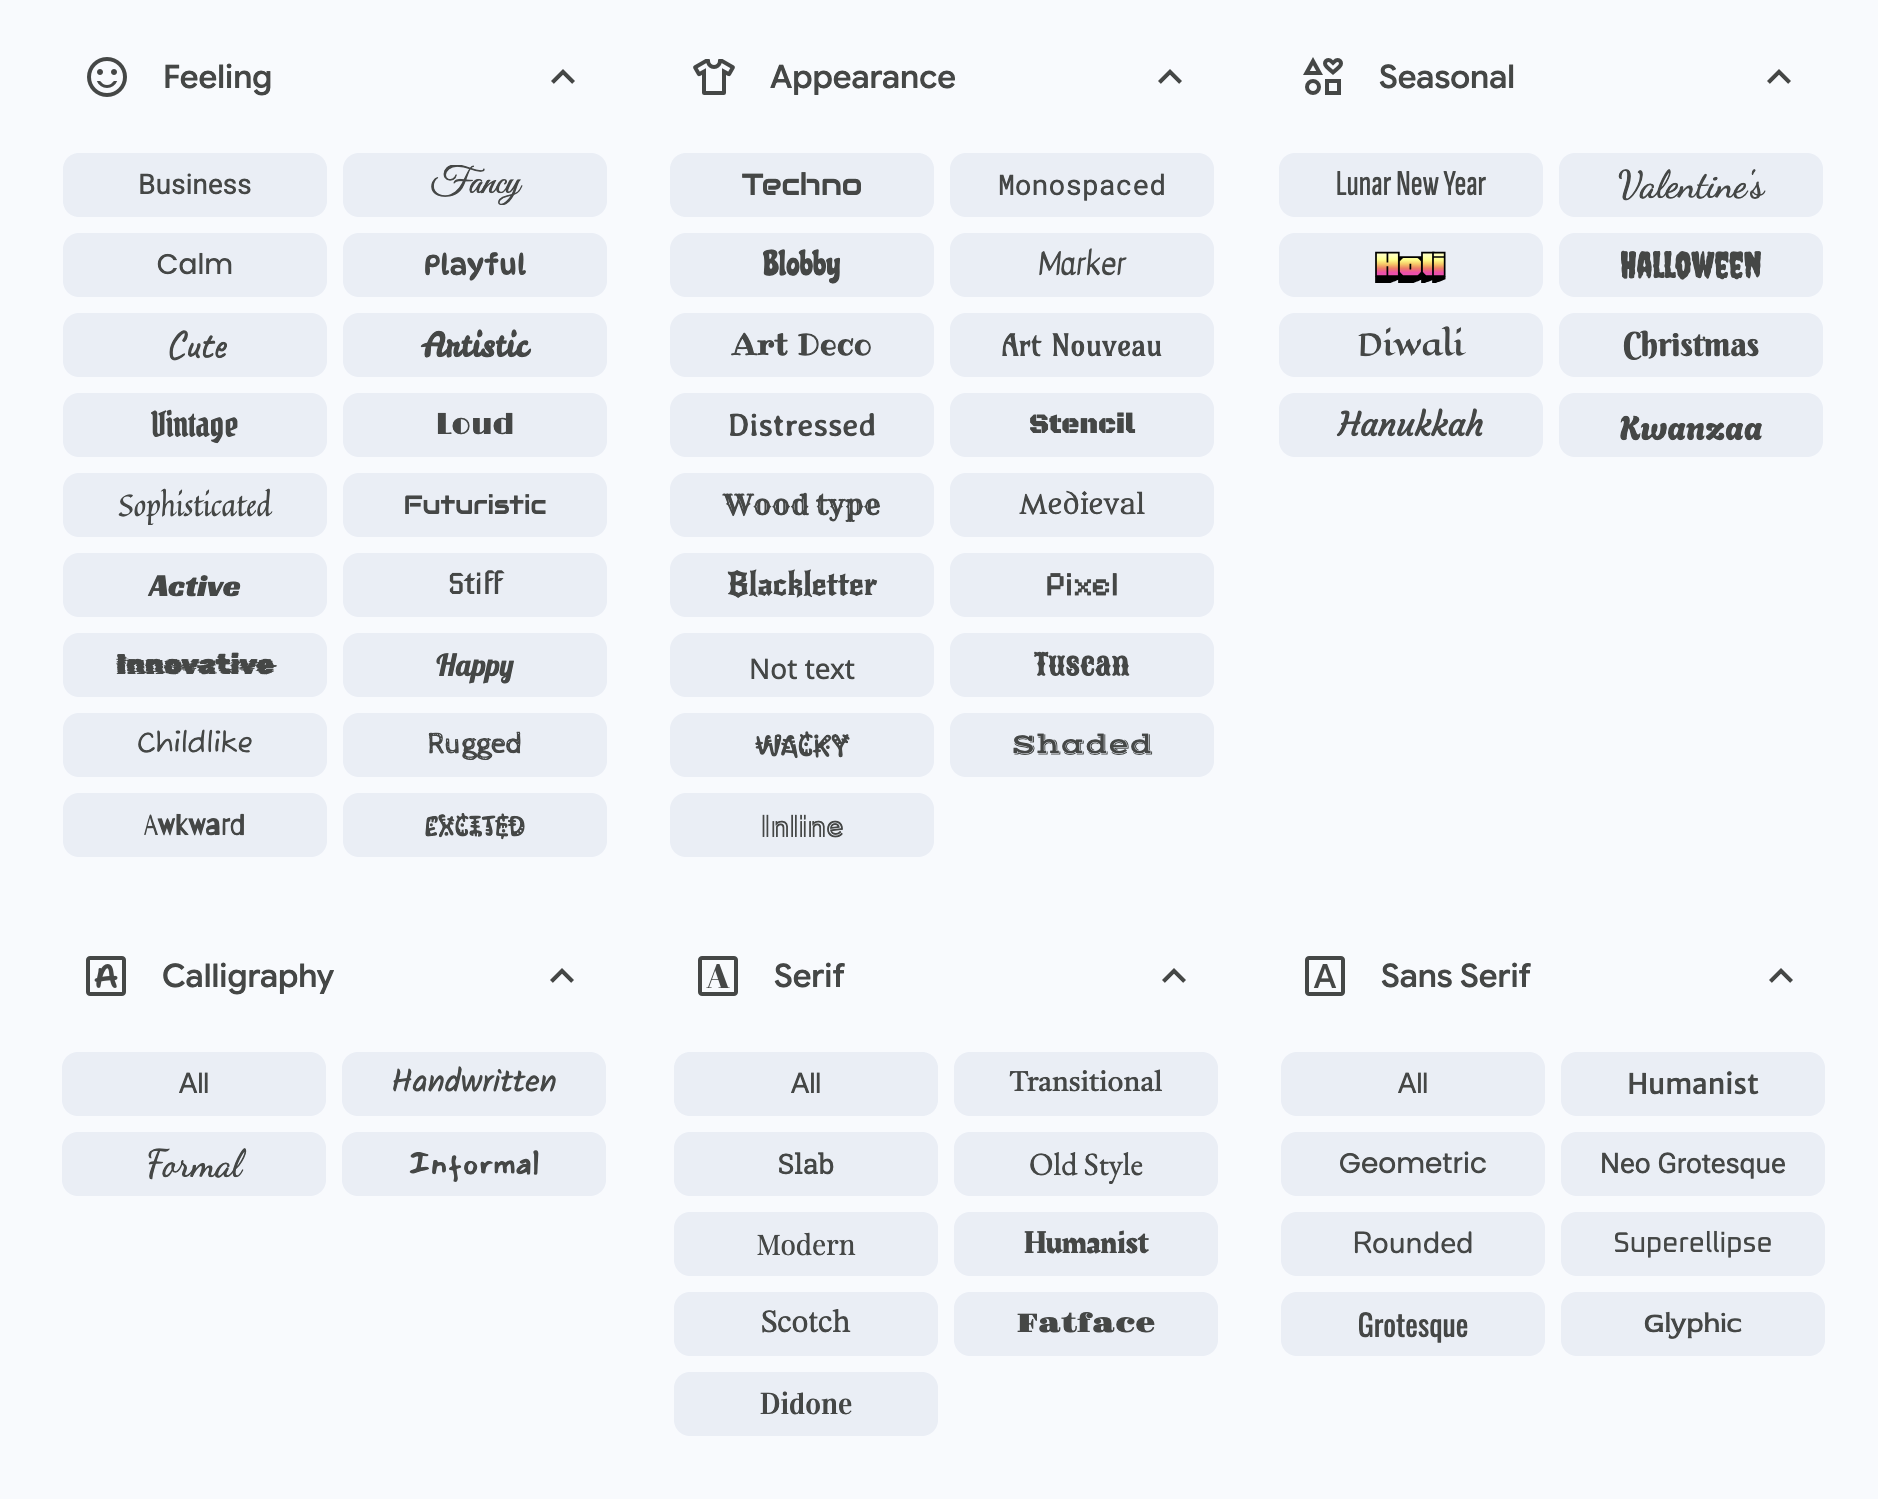
\includegraphics[width=.85\textwidth]{images/google-font-categories.png}
    \caption{Some typeface categorizations in the new Google Fonts interface}
    \label{fig:google-font-categories}
\end{figure}

The new font selection interface on the Google Fonts website\footnote{https://fonts.google.com} was released in early 2025. Whereas Google previously organized their fonts into 5 broad categories (Display, Handwriting, Monospace, Serif, and Sans Serif), their new interface introduces a much larger set of typeface categories, broken into broader parent categories (see Figure \ref{fig:google-font-categories}). In the ``Feeling" category, for example, users can filter ``Happy" fonts, ``Calm" or ``Playful" fonts, and ``Childlike" or ``Awkward" fonts. The new interface also includes appearance categories like ``Techno" or ``Art Deco," as well as holiday categories for Halloween, Hanukkah, Christmas, and Holi, among others.

% own screenshots
\begin{figure}
    \centering
    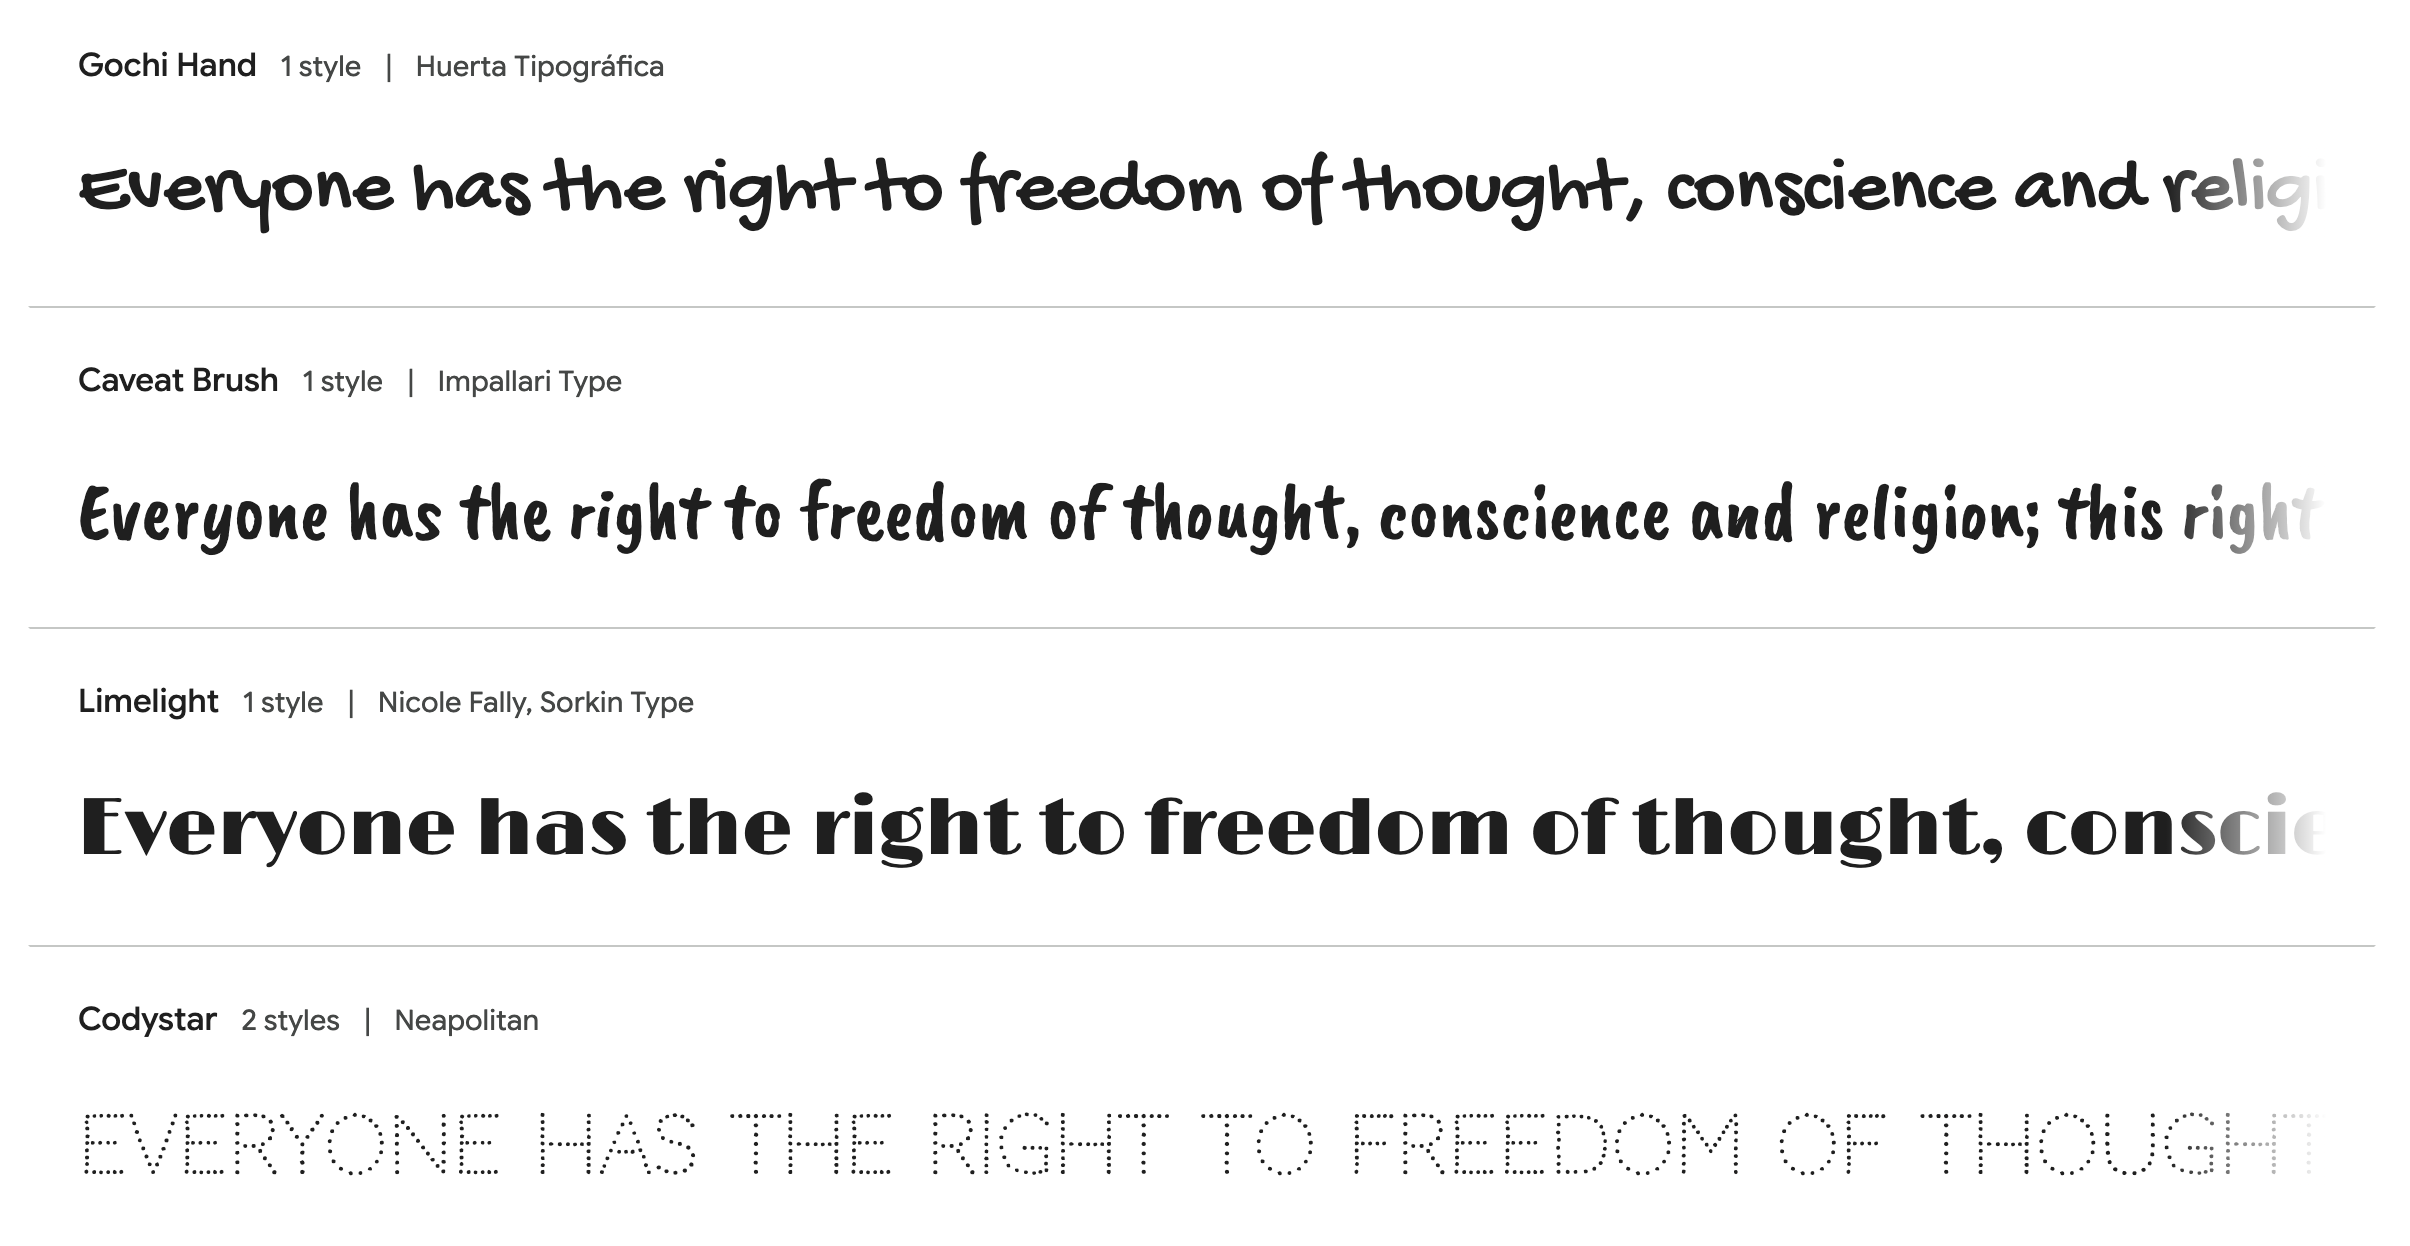
\includegraphics[width=1\textwidth]{images/google-fonts-christmas.png}
    \caption{Some of the ``Christmas'' fonts in Google Fonts do not seem very Christmassy}
    \label{fig:google-fonts-christmas}
\end{figure}

Google Font's categories break with the basic list-based interface; however, the tool has several drawbacks. For one, the user is forced to choose between discrete categories, rather than an open-ended text input, limiting their selection process to preconceived descriptors. Additionally, these categorizations are subjective; and while many of the groupings seem fairly accurate, some are questionable (such as the ``Christmas'' fonts in Figure \ref{fig:google-fonts-christmas}). Most importantly, Google has not incorporated this new font selection tool into their main Google Suite applications (Google Docs, Google Slides, and Google Sheets) where the majority of their users are choosing fonts. Most users are unfamiliar with the Google Fonts website, and therefore will not use the interface. This new font selector tool, available only from a separate website, is an interesting experiment in language-based font selection, but not yet more than that.

Canva, a popular online graphic design tool, has also experimented with a language-based font selection tool: their main design interface allows users access to select fonts via a text input field. For example, a user could type ``Modern'' and they would be presented with a wide-variety of modern-style fonts. However, while the input prompt appears open-ended, the tool actually only works for a small set of keywords; for most text input, it will either yield no results or simply return fonts whose name contains that keyword (see Figure \ref{fig:canva-font-selector}). For many unseen inputs like ``Professional,'' ``Cheerful,'' ``Ancient,'' and ``Lightweight'' the tool returns no results at all.

% own screenshots
\begin{figure}
    \centering
    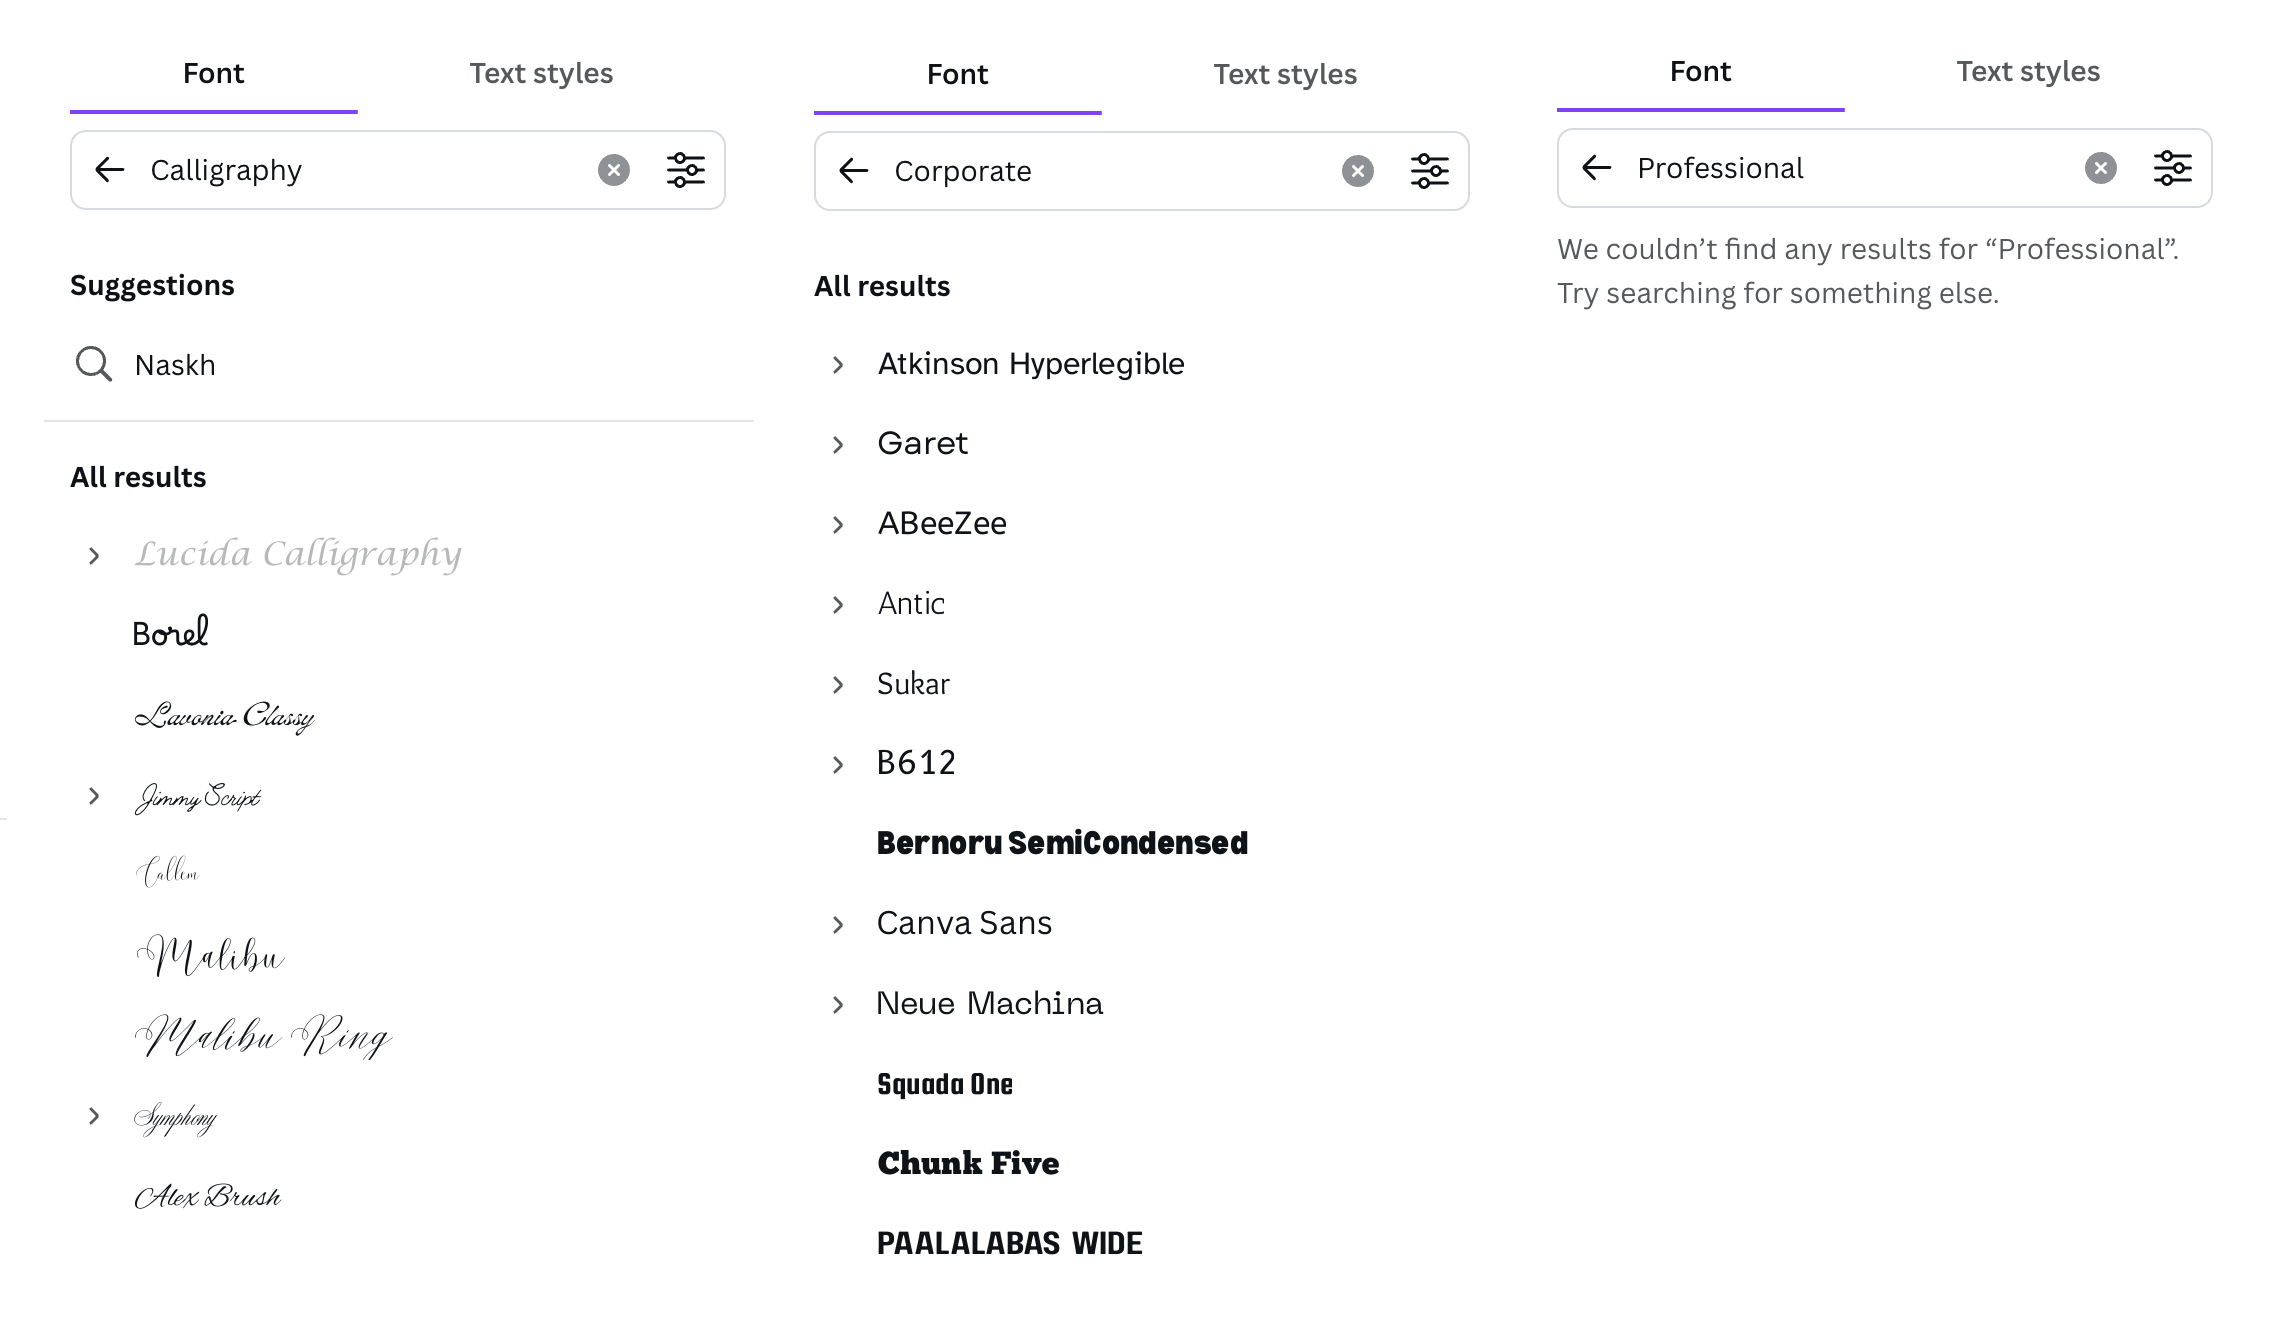
\includegraphics[width=.95\textwidth]{images/canva-font-selector.png}
    \caption{Example usages of the Canva text-based font selector tool}
    \label{fig:canva-font-selector}
\end{figure}

\subsection{Issues with Language-Based Models}

Both of the above tools use keyword descriptors for font selection, one with predetermined style categories (Google Fonts) and the other with an open-ended search box which, in reality, allows only a limited set of keywords as input (Canva). The direction of this approach, however, is not a bad one. Language is one of the ways in which humans fundamentally conceive of the world, including with respect to visual style. Especially given the popularization of Large Language Models (LLMs) and chatbots, there is certainly an open space for innovation with language-based font selection. However, there are a couple key problems with creating these language-based font selection models. First of all, visual style is quite subjective: one user might find a certain font ``wacky'' while another might find that font ``sad'' or ``disgusting.'' A font which one user finds ``professional'' another might find ``playful.'' Building a language-based model for font selection should therefore account for user subjectivity in its recommendations. Secondly, there is a relative lack of datasets which connect typefaces to language-based style characteristics. Shaikh et al.\ \cite{shaikh2006} perform an online study with hundreds of participants to generate a dataset of only 20 fonts and 15 style adjectives. O'Donovan et al.\ \cite{odonovan2014} generate a larger dataset of 200 fonts and 31 style adjectives, but this is still relatively small when compared with the hundreds of thousands of available fonts and the many possible dimensions of style. For this project, we mostly avoid the issue of language-based font selection, and rather focus on the use of unsupervised neural models in building useful style-based font selection tools.

\subsection{An Analogue: Color Selection}

A useful analogue when considering the issue of typeface selection is another common problem in graphic design: color selection. The field of color selection has produced a much wider range of selection interfaces, which suggests a potential for a much more diverse set of font selection tools. Figure \ref{fig:basic-color-picker} shows a common, basic color selection tool containing several ways to interact with its many available colors: sliders, numeric input, and a 2-dimensional gradient. Color can be represented using a 4-dimensional basis called RGBA: red-value, green-value, blue-value, and transparency-value. The first three are based on a hexadecimal scale, allowing values between 0 and 255, while the transparency value is constrained between 0 and 1. By representing color using a multi-dimensional basis, users have an intuitive, finer-grained control over the color selection process. This is more useful than, say, selecting from an alphabetized list of colors (Apricot, Aquamarine, Baby Blue, Canary Yellow...), which---similar to an alphabetized list of fonts---does not provide users with a very meaningful way to navigate the dimensions of color. There are many other popular tools for color selection: Adobe Color, for example, utilizes a popular color-wheel tool, and additionally includes features to change color basis (CMYK and RGBA are the most common color bases, but other more obscure ones exist), pick a set of colors based on a particular harmony (Monochromatic, Triad, Complementary, e.g.), and save colors to a library for later access (see Figure \ref{fig:adobe-color}).

% from rgbacolorpicker.com
\begin{figure}[]
    \centering
    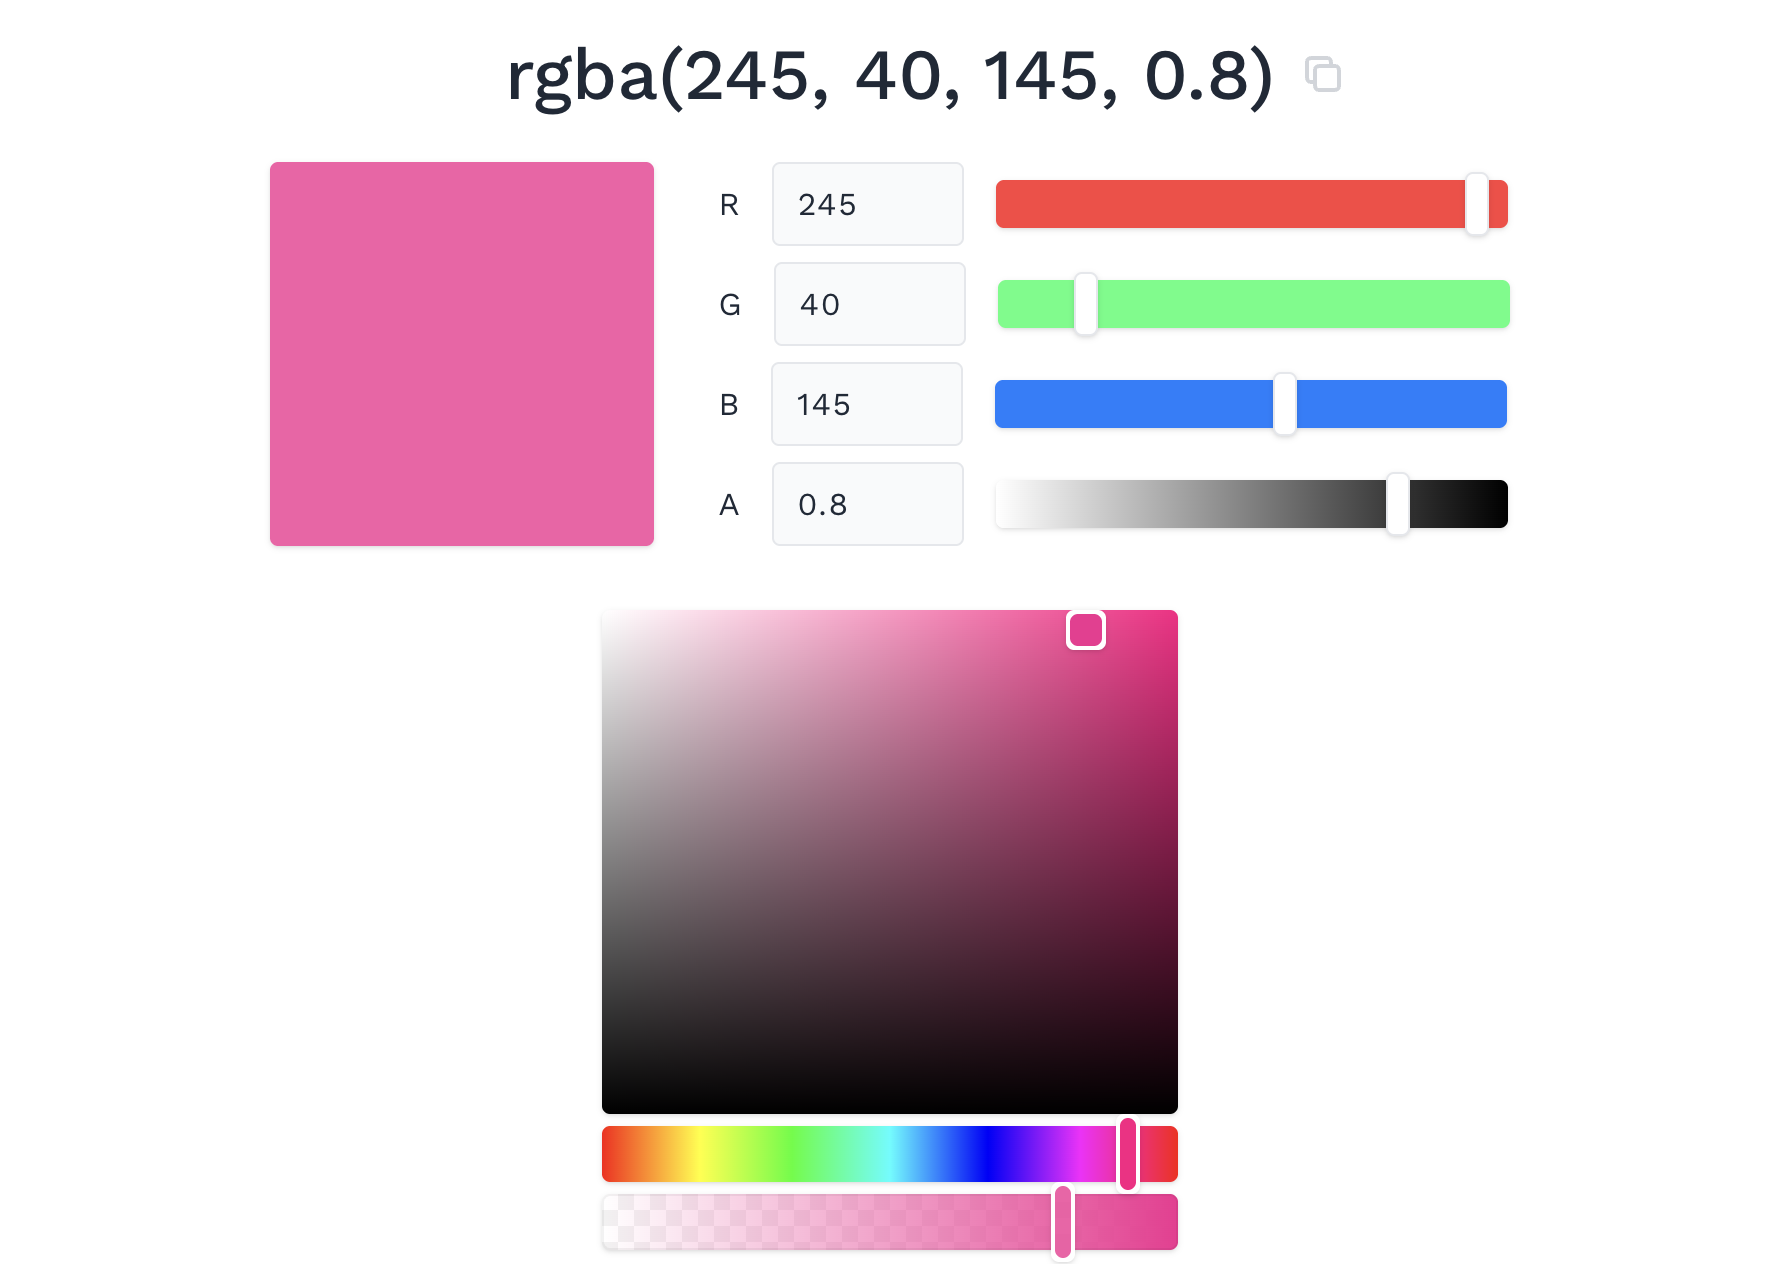
\includegraphics[width=0.8\textwidth]{images/basic-color-picker.png}
    \caption{A basic color selection interface with gradient, numeric, and slider controls}
    \label{fig:basic-color-picker}
\end{figure}

% from color.adobe.com
\begin{figure}[]
    \centering
    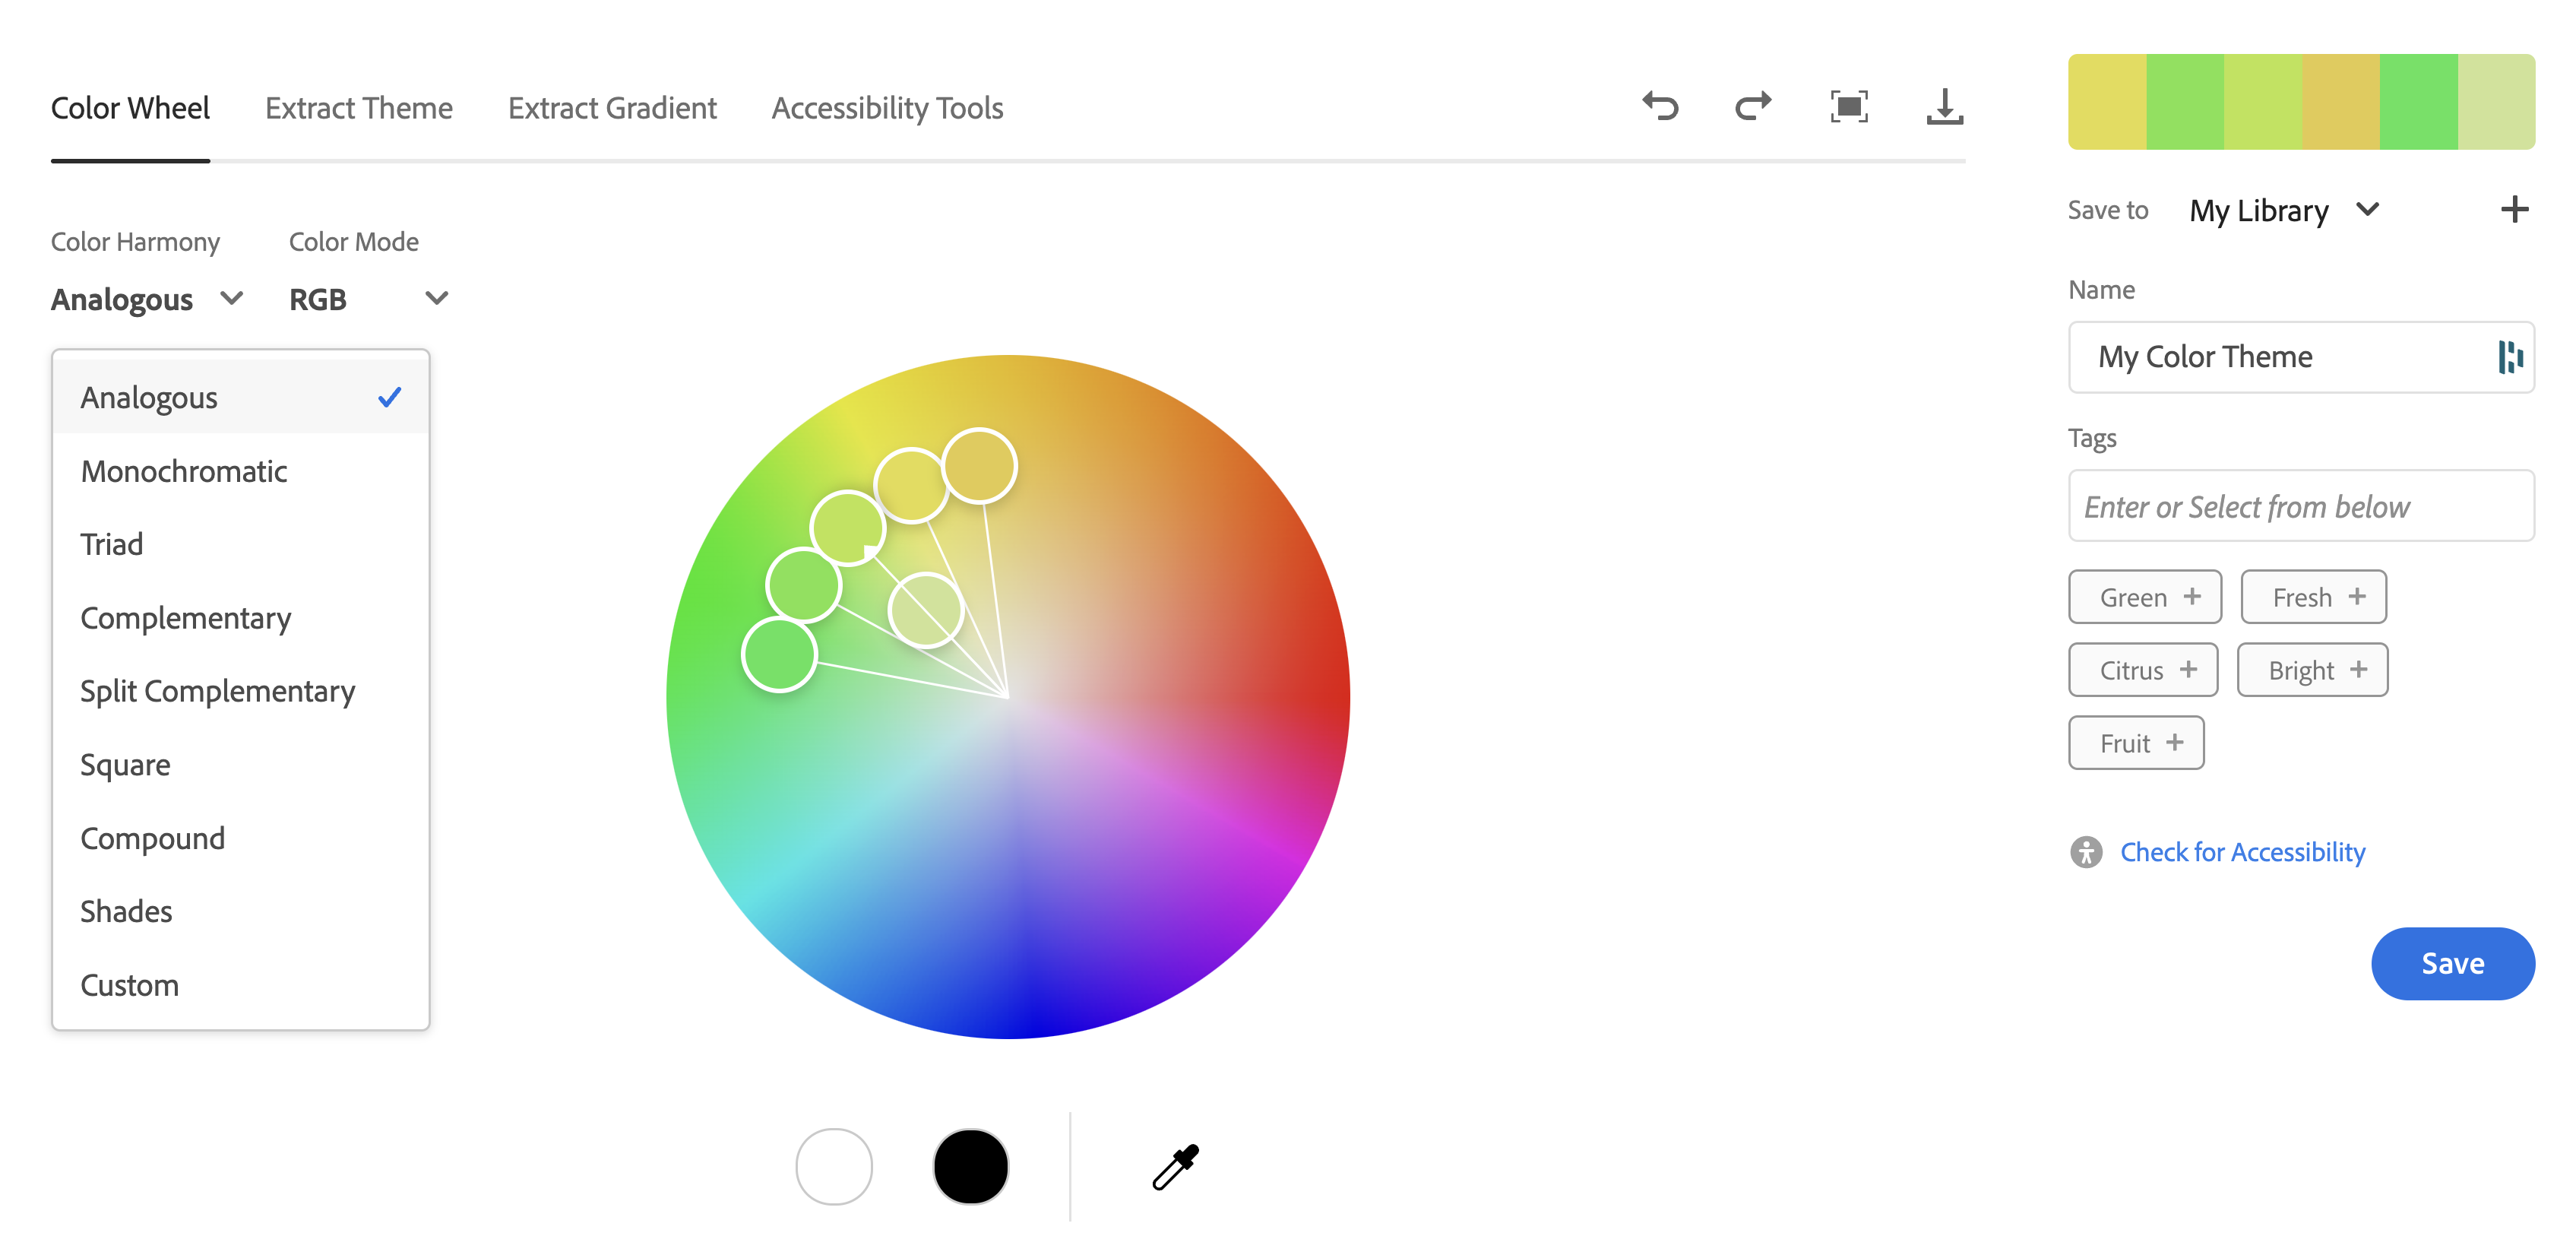
\includegraphics[width=\textwidth]{images/adobe-color.png}
    \caption{Adobe Color selection interface, with a color wheel, multiple color bases, color harmony-based selection, and the ability to save colors}
    \label{fig:adobe-color}
\end{figure}

The wide range of diverse color selection interfaces and color bases suggests a potential for similarly-diverse, useful selection tools for typeface which provide control over the many dimensions of typeface style. While typefaces and their style cannot be decomposed as easily as color, their style \emph{can} be represented using a vector basis---as we will show in subsequent chapters---and building selection tools on a vector space of style dimensions could allow users greater control in typeface selection---similar to the level of control users have in color selection. Imagine, perhaps, a gradient of fonts, or sliders which control different aspects of font style. These ideas are not farfetched: as our research will show, neural networks---specifically autoencoder-like neural network models---can be used to distill quantitative style encodings from font image data, which provides a foundation upon which to build better style-based font selection tools.

\section{Autoencoders}

As previously stated, we hypothesize that neural networks might provide a useful foundation for font selection tools by generating typeface style encodings. More specifically, we focus on autoencoder and autoencoder-like models in our neural network design. This section provides background on the autoencoder model and why autoencoder-like neural networks might provide a useful foundation for creating style-based font selection tools.

\subsection{Autoencoder Model}

The autoencoder \cite{rumelhart1986} is a specific type of neural network trained to exactly reconstruct its input. The model is composed of two parts: an encoder, which transforms the input to an intermediate representation (usually smaller than the input representation) through a series of linear and nonlinear operations; and the decoder, which transforms the intermediate representation back to the original input size. By minimizing the loss of this neural network during training, the encoder learns to condense the input data for later reconstruction, and the decoder learns to reconstruct that data based on the intermediate representation generated by the encoder.

% from Bank et al. "Autoencoders" DO I NEED TO CITE THIS?
\begin{figure}[h]
    \centering
    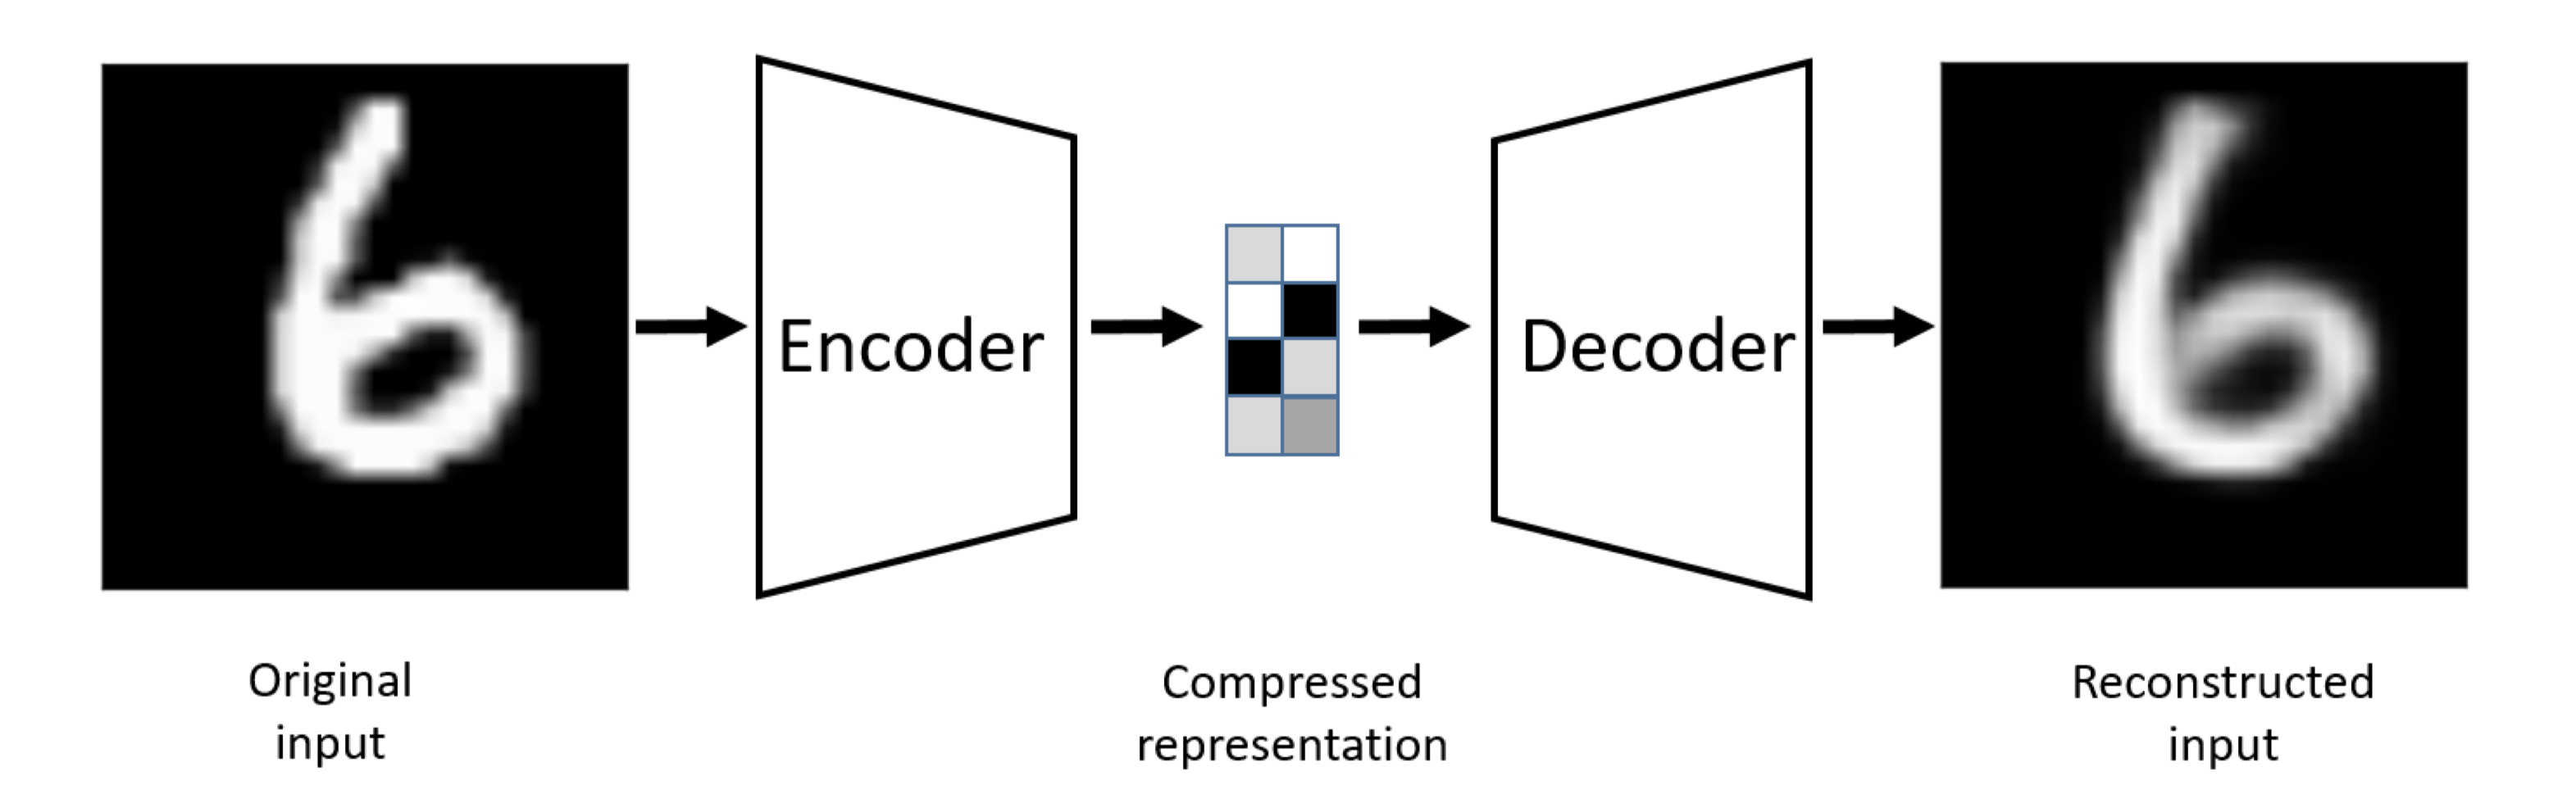
\includegraphics[width=\textwidth]{images/autoencoder-model.png}
    \caption{Basic autoencoder model applied on an image from MNIST, a dataset of handwritten images widely-used for image classification tasks \cite{lecun1998}}
    \label{fig:autoencoder-model}
\end{figure}

The autoencoder model may seem of little use---why would I want to reconstruct data which I already have? The main goal of an autoencoder, however, is not the final reconstructed output but rather the intermediate representation---which distills the essentials of the input. In order for the decoder to be able to accurately reconstruct input data which it has never seen, the encoder part of the model must encode an intermediate encoding that captures enough salient aspects of the input for the reconstruction stage. Thus, the autoencoder's intermediate representation tends to be a rich and concise summary of the input. In our research, we leverage these encodings as a proxy for typeface style. Bank et al. \cite{bank2021autoencoders} write:

\begin{quote}
    ...the goal of autoencoders is to get a compressed and meaningful
    representation. We would like to have a representation that is meaningful to us...
\end{quote}

In order to create meaningful representations, however, some steps must be taken to avoid simply learning the identity function. To accomplish this, the autoencoder model usually includes a bottleneck---meaning that the encoder must compress the input before giving it to the decoder (see Figure \ref{fig:autoencoder-model}). Therefore, the model \emph{cannot} simply learn the identity function and must learn to produce a useful, condensed version of the input. In our case, the purpose of training an autoencoder model to reconstruct font data is not the output images, but rather these intermediate encodings. Importantly, while a bottleneck is the most common technique to achieve this effect, other methods such as adding Gaussian noise \cite{bank2021autoencoders} can be used instead of or in addition to a bottleneck.

\subsection{Variations on the Autoencoder}

There have been many variations on this basic autoencoder model \cite{michelucci2022}. While the basic autoencoder is unsupervised, it is possible to feed additional data into the autoencoder, such as data labels, in order to coerce the model to ignore these aspects of the input data in the construction of an intermediate representation. (In our research, we employ this method to disentangle \textit{content}---i.e. the character being represented---from \textit{style.}) Another alteration of the original autoencoder is the variational autoencoder (VAE) model \cite{kingma2013}, which uses probabilistic distributions to improve autoencoder performance, especially with respect to generative tasks. Rather than encoding an explicit intermediate encoding, VAEs encode the parameters of a multi-dimensional Gaussian distribution which represents the probabilistic space of the intermediate encoding. The decoder then samples randomly from the distribution and proceeds with the decoding task. This probabilistic model is especially useful in generative tasks, when the goal is to generate new content (e.g. to generate a new character in a font), but the continuous latent space encoded by VAEs can also be directly used, as in our case, as a compact representation of salient input properties like visual style.

\section{Previous Work}

There has been previous scholarly on improving font selection interfaces, especially based around font inference models. This section explores some of these models, one based on crowdsourced data, and the others on neural inference models. Both of these approaches have informed our research, but the neural inference models have particularly influenced the models we have built. Particularly, we adapt the Srivatsan et al. model \cite{srivatsan2020} in our work and use the style encodings trained by the model to build our typeface selector tool.

% own screenshots
\begin{figure}
    \centering
    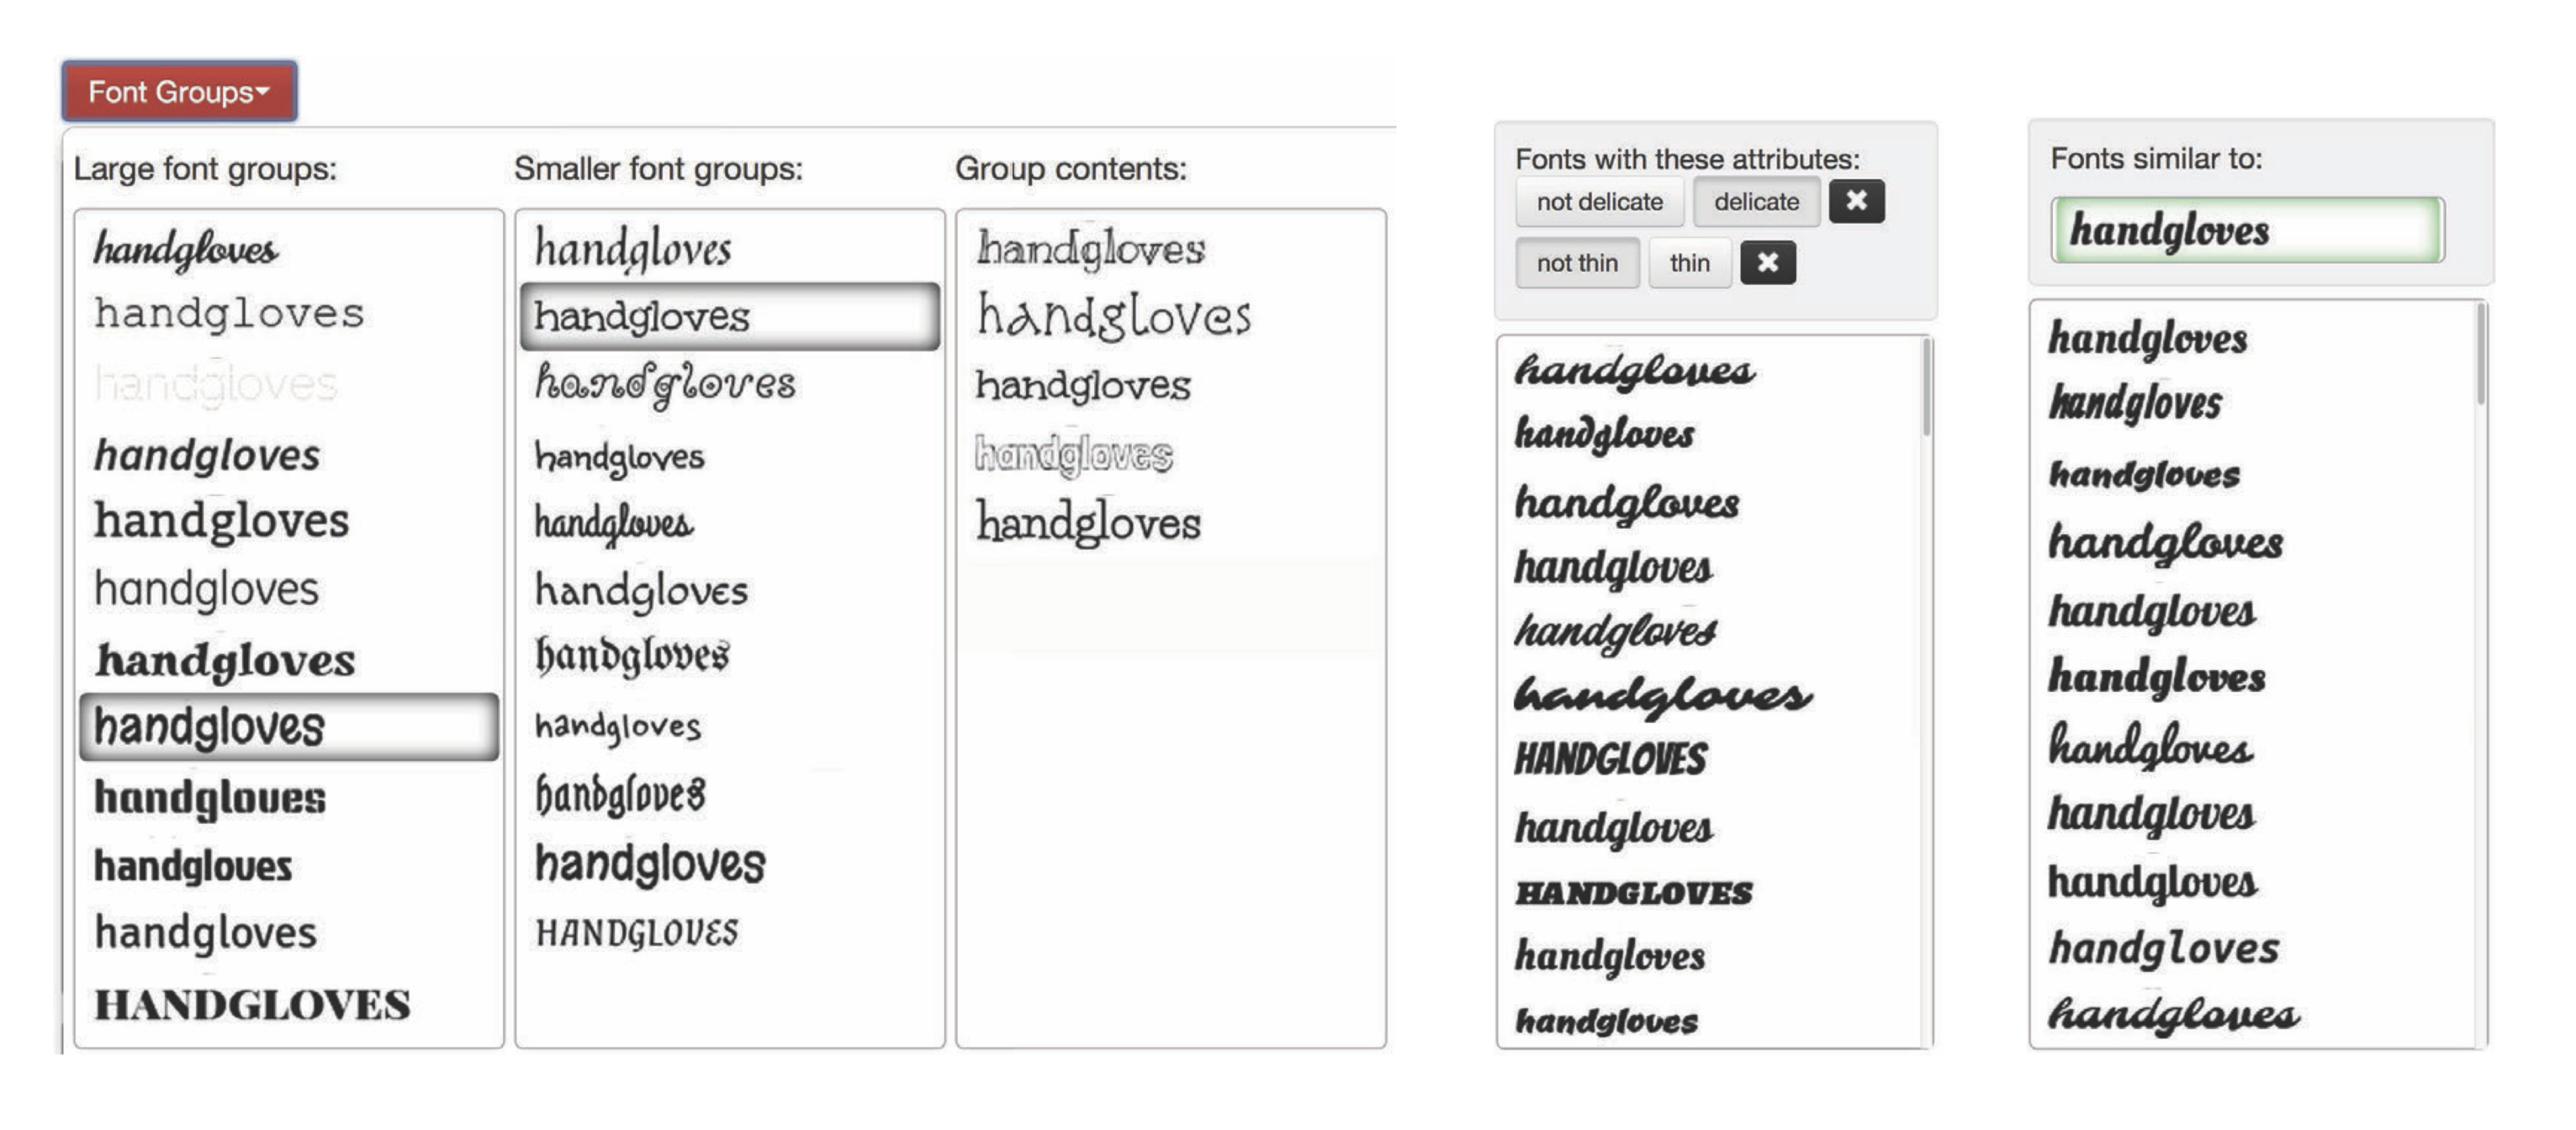
\includegraphics[width=1\textwidth]{images/odonovan-interfaces.png}
    \caption{Group Interface, Attribute Interface, and Search-By-Similarity selection tools from O'Donovan et al. \cite{odonovan2014}}
    \label{fig:odonovan-interfaces}
\end{figure}

\subsection{Crowdsourced Models}

O'Donovan et al.\ \cite{odonovan2014} proposes three novel font-selection interfaces, built on crowdsourced data from Amazon Mechanical Turk (MTurk): one based around verbal attributes such as ``formal,'' ``friendly,'' or ``legible'' called Attribute Interface; another which clusters fonts hierarchically based on visual similarity, called Group Interface; and a third, to be paired with the other two methods, which provides users with a list of similar fonts to the current selection, called Search-By-Similarity (see Figure \ref{fig:odonovan-interfaces}). The researchers built these models on crowdsourced data collected through MTurk: they prompted users to answer questions such as ``Which of these two fonts is more strong?'' or ``Which of these fonts is more silly?'' to collect attribute data, and asked questions like ``Which of these two fonts—Font B or Font C—is more similar to Font A?'' in order to build similarity data. The Group Interface model splits fonts into large categories based on similarity, creating a tree-like font selection tool where users can progressively narrow down their font selection task. The Attribute Interface, similar to the Google Fonts and Canva interfaces, attaches adjective descriptors to fonts, which is helpful as humans tend to conceptualize style based on verbal descriptors. Finally, they use the similarity data to create their Search-By-Similarity tool, to be used in conjunction with the other two methods: given a selected font, which fonts are most similar according to other users? This provides an important principle for typeface selection: if a user is looking to select a font based on style characteristics, it is useful to see other fonts that are similar according to other users. All of these tools are potentially useful ways to navigate typeface selection by means of style, but it should be noted that basing these attributes and similarity scores on crowdsourced data means that these tools may not align with every user's subjective sense of style. O'Donovan et al.\ additionally conducted user studies, also on MTurk, presenting users with either font matching or design tasks to evaluate their interfaces against a baseline font selector tool. The researchers found positive results for their novel font selection tools: participants were three times more likely to succeed in a font-matching task using any of the three proposed interfaces compared with a basic list-based interface, and they also found a small statistically significant improvement in user performance on the design task between their selection interfaces and the baseline.

\subsection{Inference Models}

There has also been some effort to build inference models around font character images, sometimes with the explicit purpose of building better user-interface for font selection. Cho et al.\ \cite{cho2022}, for example, builds a model with the explicit goal of generating latent space encodings of glyphs which are easily differentiable based on their font. They describe their model design as such:

\begin{quote}
    For the discriminative representation of a font from others, we propose a paired-glyph matching-based font representation learning model that attracts the representations of glyphs in the same font to one another, but pushes away those of other fonts.
\end{quote}

\begin{figure}
    \centering
    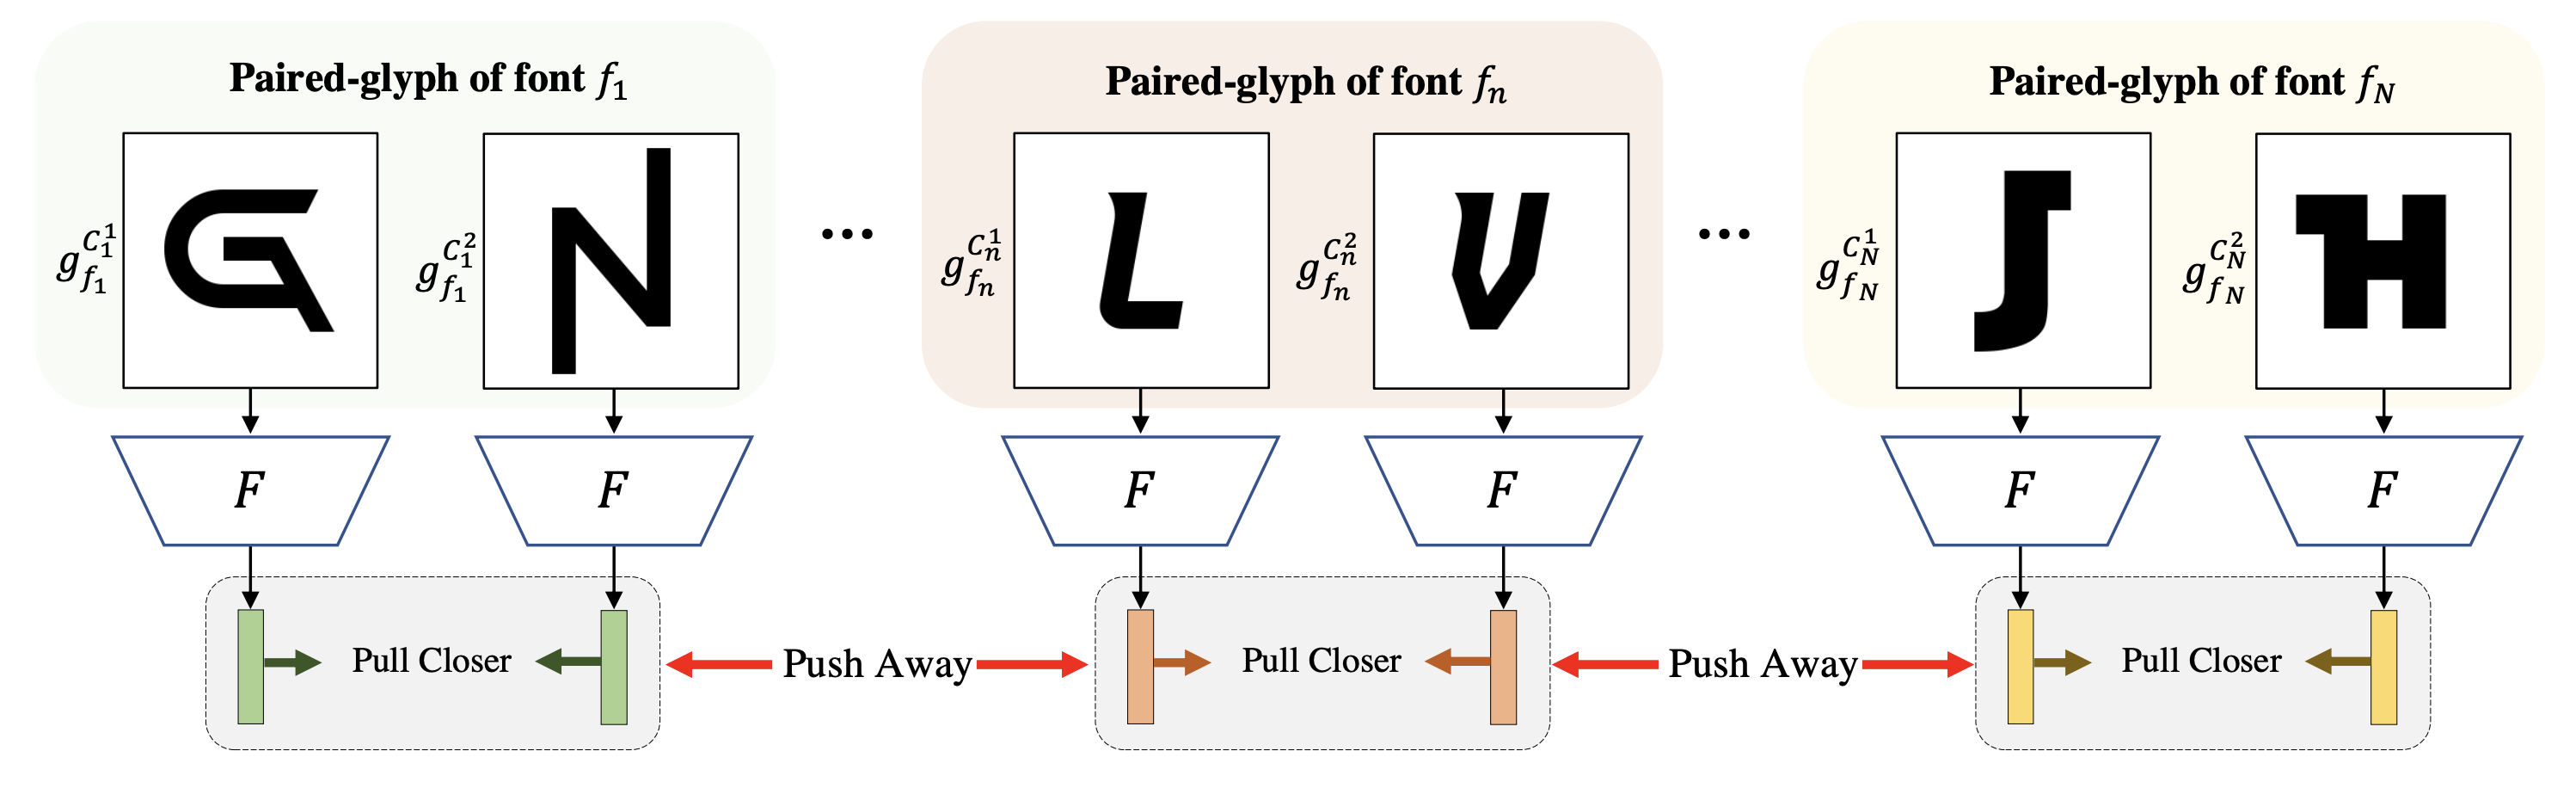
\includegraphics[width=1\textwidth]{images/cho-paired-glyph.png}
    \caption{Paired-glyph matching in Cho et al. \cite{cho2022}}
    \label{fig:cho-paired-glyph}
\end{figure}

Their paired-glyph matching, shown in Figure \ref{fig:cho-paired-glyph}, involves selecting random pairs of glyphs and training the model to prefer a low cosine similarity (more similar) between the representations if the glyphs are characters in the same font, and a high cosine similarity (less similar) if the glyphs come from different fonts. While Cho et al.\ succeeds in their goal of clustering the latent space representations of glyphs by typeface, it is unclear how well these encodings will represent the stylistic aspects of typeface. Notably, the training technique focuses on decreasing the cosine similarity of encodings for characters of different typefaces, but it does not seem to have a mechanism to actually consider the style of a character or typeface. Rather, the training data for their model is essentially the \emph{name} of a font. As Figure \ref{fig:cho-latent-space} shows, their model performs well at discriminating character style encodings based on font---their model effectively clusters characters according to their typeface, denoted by point color---but the model space may not represent meaningful dimensions of typeface style (weight, size, serif) beyond simply separating fonts which are not identical.

\begin{figure}[]
    \centering
    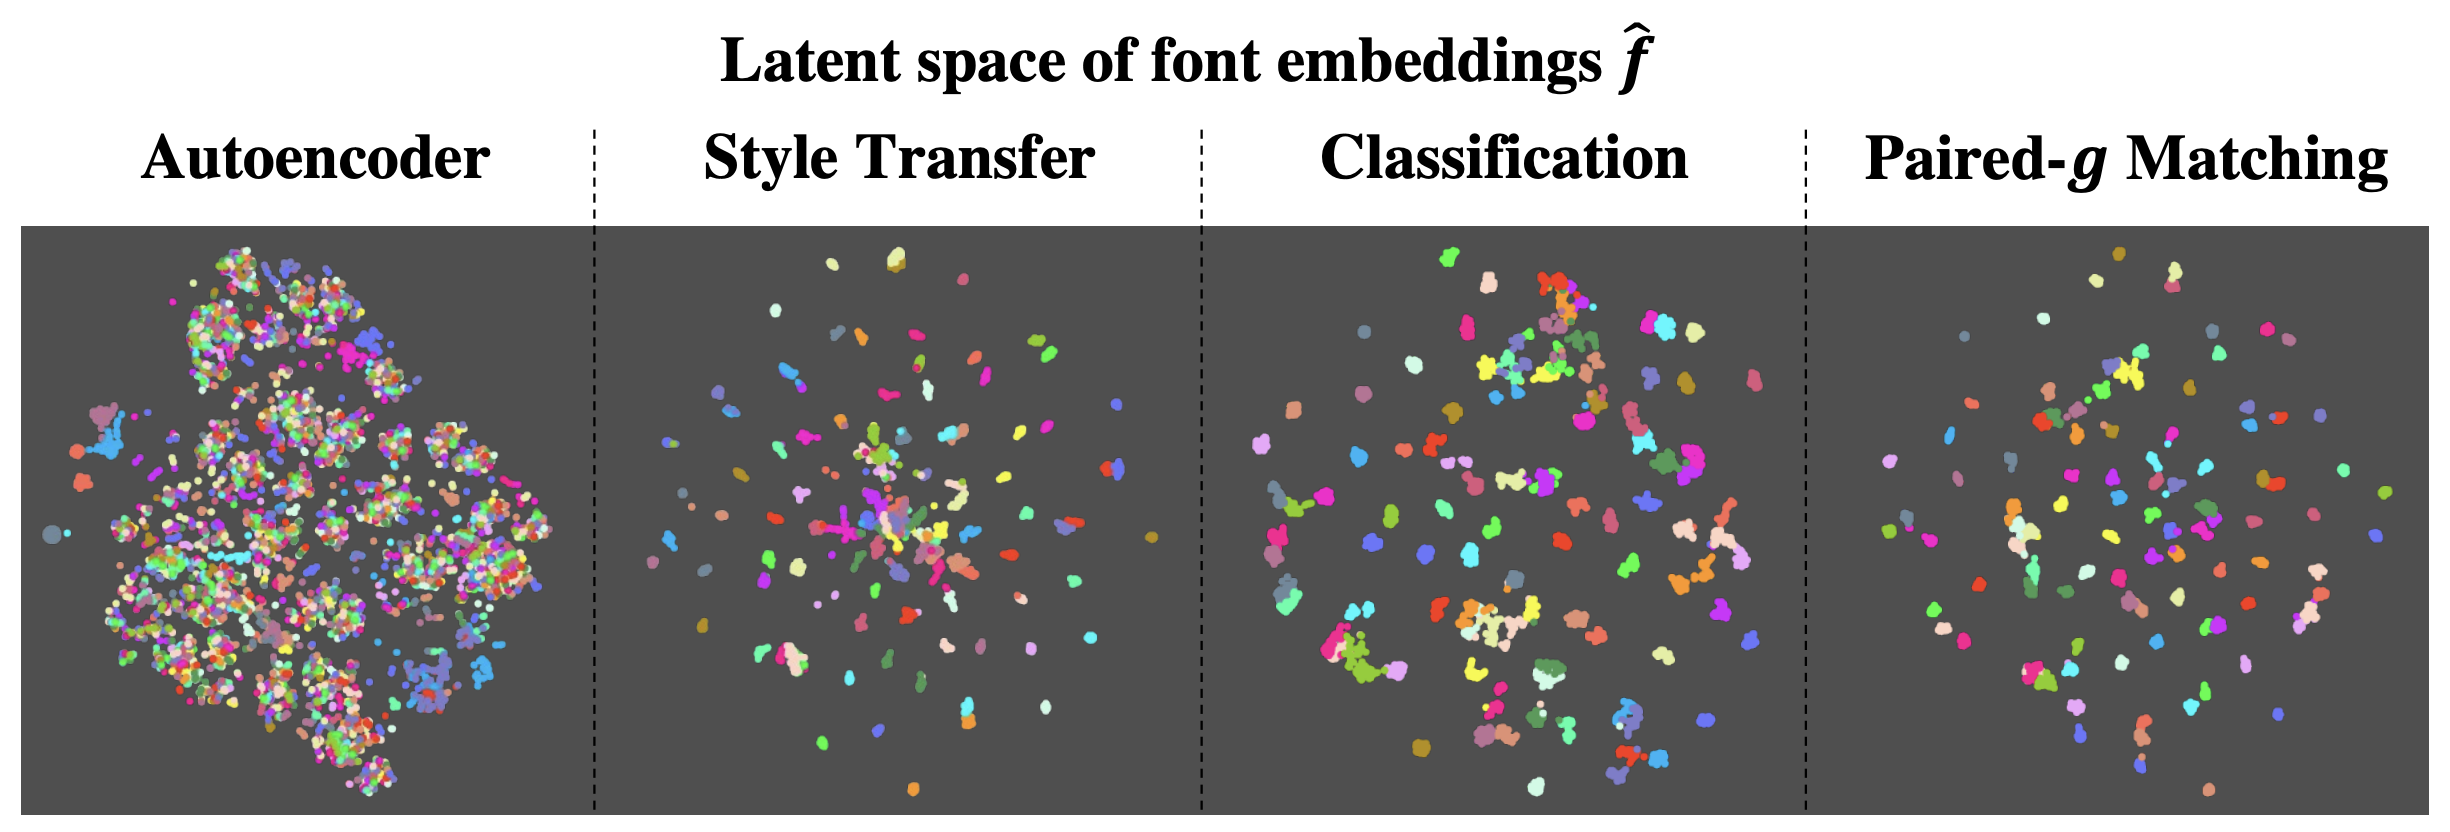
\includegraphics[width=1\textwidth]{images/cho-latent-space.png}
    \caption{Latent space of style embeddings across model techniques in Cho et al. \cite{cho2022}, with color representing the typeface of a given character style encoding}
    \label{fig:cho-latent-space}
\end{figure}

Relevant to our work is their evaluation of different model architectures for generating style encodings. As shown in the latent space maps in Figure \ref{fig:cho-latent-space}, they employ three different model architectures in addition to their paired-glyph matching: the basic autoencoder model, style transfer (generating another character in the same font given an input character), and classification (predicting which font is represented in a glyph). There is an overlap in some of their model choices and ours (namely, autoencoder and style transfer), and the figure they provide is useful in visualizing the typeface-clustering effectiveness of these various models.

\begin{figure}[h]
    \centering
    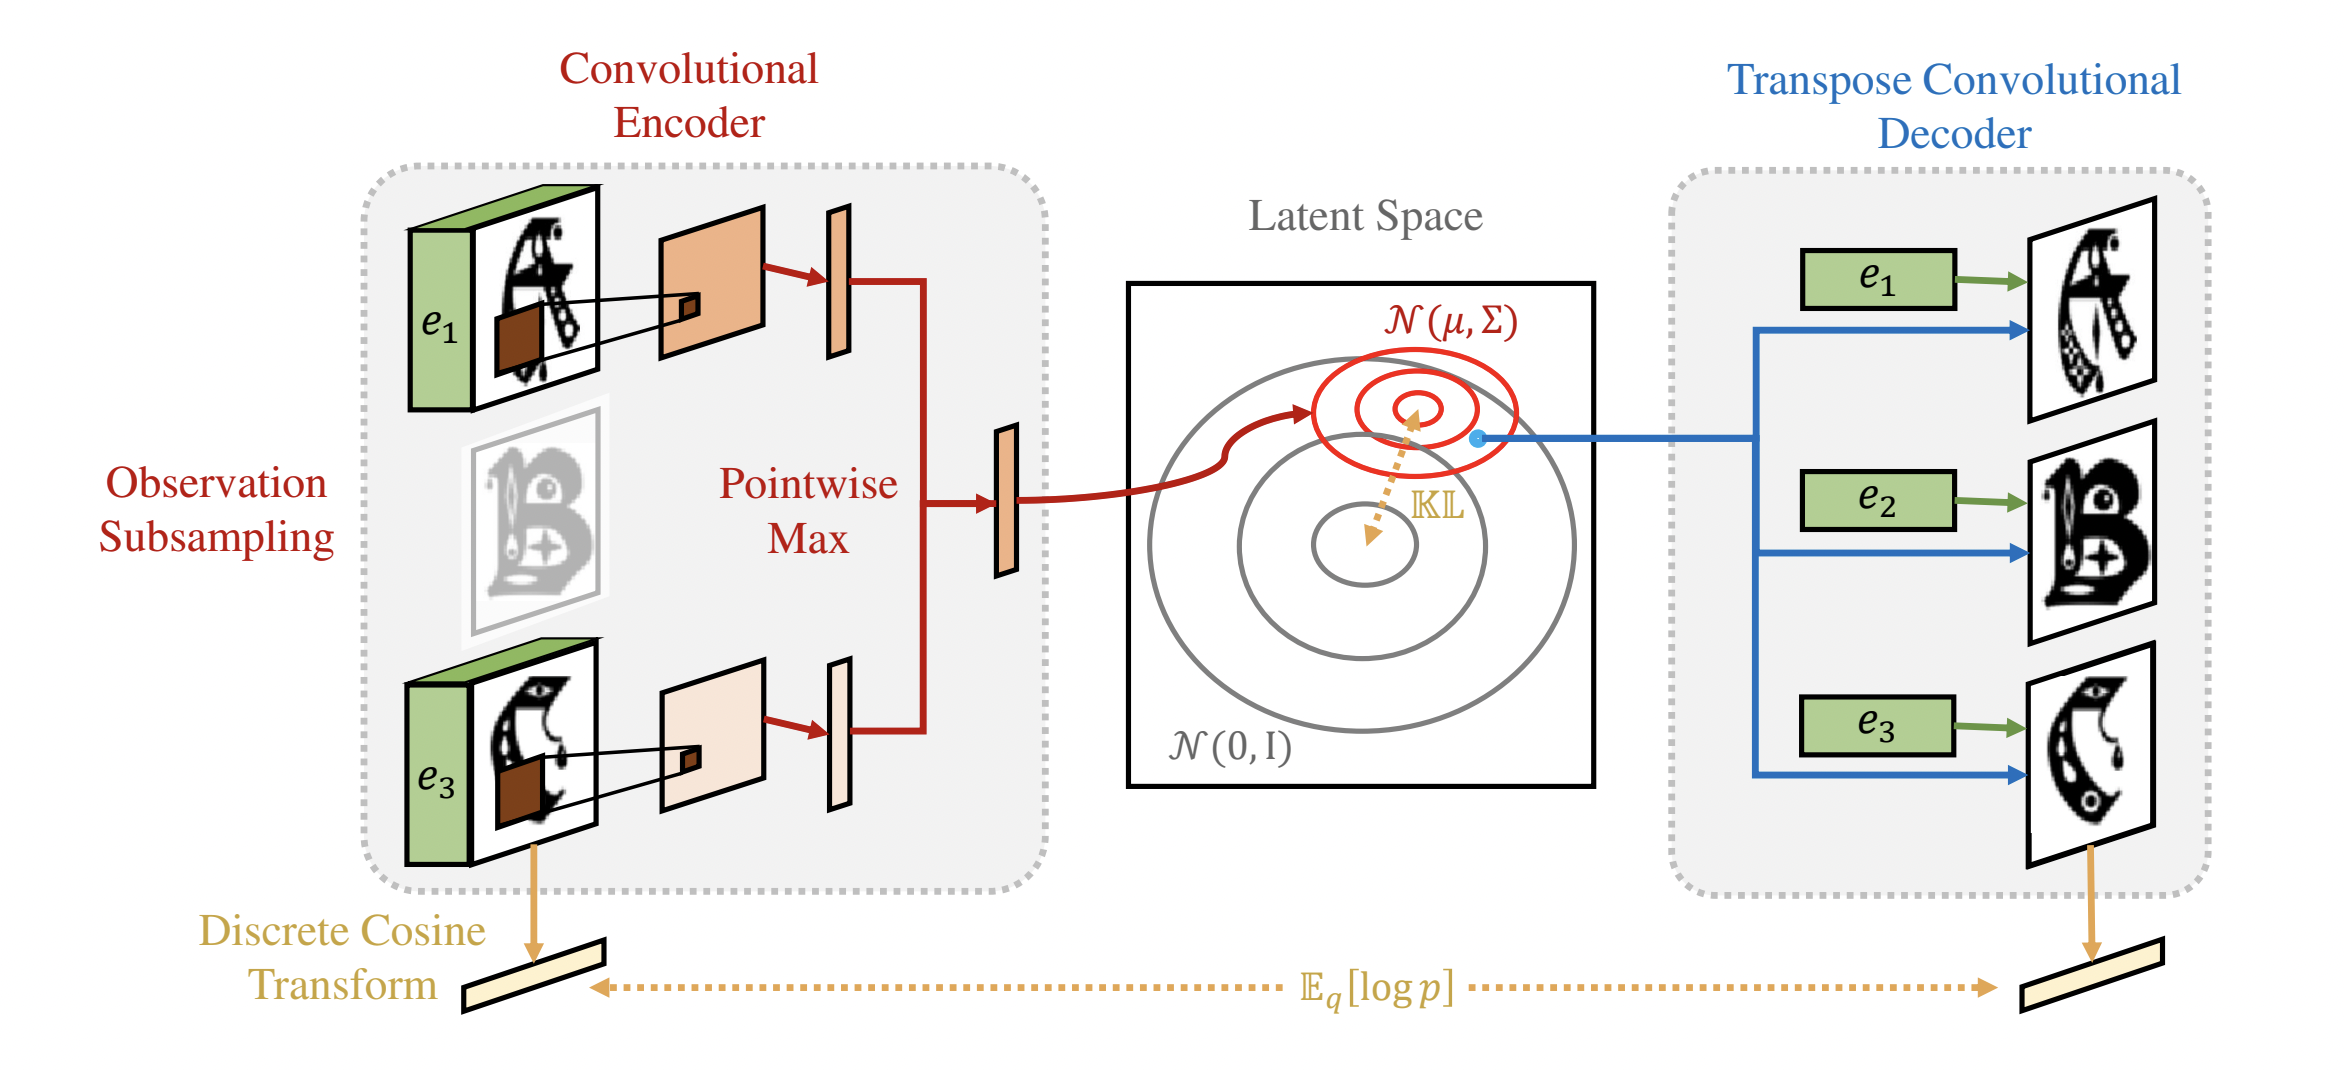
\includegraphics[width=1\textwidth]{images/srivatsan-model.png}
    \caption{Generative process of model Srivatsan et al.}
    \label{fig:srivatsan-model}
\end{figure}

Srivatsan et al.\ \cite{srivatsan2020} introduce a training method based on latent probability space and a tensor factorization approach well-founded in past literature \cite{freeman1997,tenenbaum2000,vasilescu2002,tang2013}. Their model explicitly seeks to disentangle style and content—to encode the typeface style of a glyph as separate from the actual character it represents. The model architecture, shown in Figure \ref{fig:srivatsan-model}, convolutionally encodes a probabilistic encoding of a font given its complete character glyph set (with a chosen number missing) and corresponding character embeddings, and uses that latent probability vector along with a given character embedding to reconstruct the missing glyphs. Their model is particularly effective at reconstructing glyphs, when compared to peer models, and it also succeeds against a state-of-the-art peer model \cite{azadi2017} when evaluated by humans on Amazon Mechanical Turk. The model additionally yields high quality style encodings, with similar fonts having similar encodings in the model space. Figure \ref{fig:srivatsan-latent} shows a t-SNE projection of their model latent space with ``A'' glyphs displayed at each centroid given k-means clustering ($k=10$). These centroids are representative of the typeface styles existing at the given area of the t-SNE plot. Lastly, Srivatsan et al. find that, qualitatively, their model seems to effectively recreate many important aspects of character style including shape, shadow, and texture.

\begin{figure}[]
    \centering
    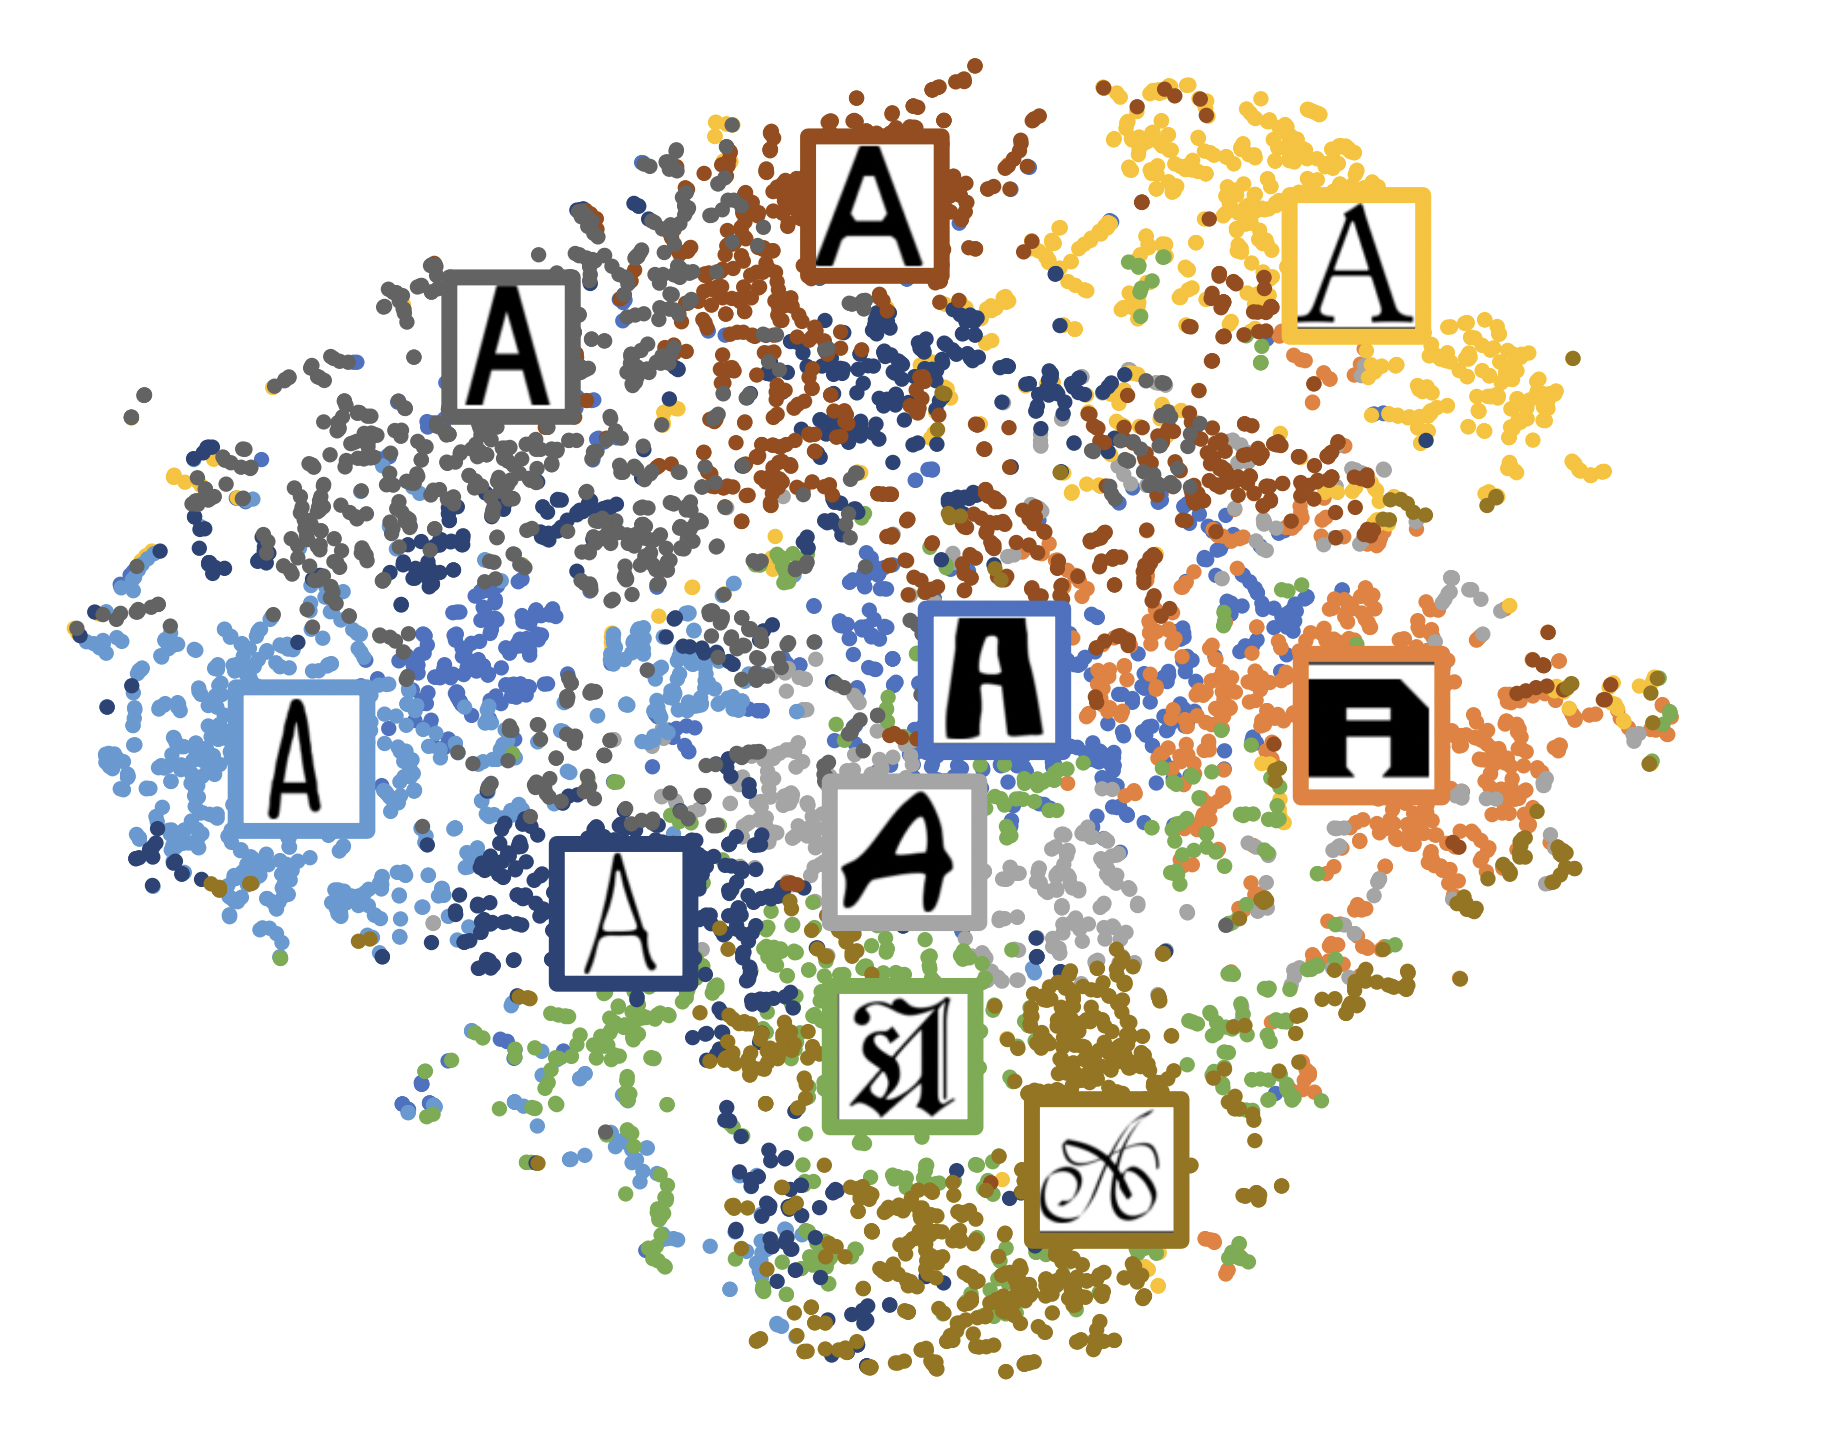
\includegraphics[width=.7\textwidth]{images/srivatsan-latent.png}
    \caption{t-SNE projection of latent font variables in Srivatsan et al.\ with centroids}
    \label{fig:srivatsan-latent}
\end{figure}

As previously stated, we chose to adapt the Srivatsan model in our research, porting it to a more recent version of Python (3.13) and PyTorch (2.5.1) and training the model on a larger dataset, comprised of the model's original training data, preinstalled Apple fonts, and the set of fonts available from the Google Fonts repository. We implement this model, along with two of our own models, and compare their respective style encodings in the following sections.